\documentclass[stu,12pt,floatsintext]{apa7}

% =========================
% PAQUETES
% =========================
\usepackage[spanish]{babel}
\usepackage[utf8]{inputenc}
\usepackage[T1]{fontenc}
\usepackage{csquotes}
\usepackage{amsmath}
\usepackage{graphicx}
\usepackage{booktabs}
\usepackage{longtable}
\usepackage{array}
\usepackage{setspace}
\usepackage{float}
\usepackage{caption}
\usepackage{url}
\usepackage{enumitem}

% =========================
% CONFIGURACIÓN APA 7
% =========================
\onehalfspacing
\setlength{\parindent}{0.5in}

% =========================
% DATOS DEL DOCUMENTO
% =========================
\title{Eranthia: Dungeon Crawler Patterns\\
Especificación de Requerimientos, Casos de Uso,\\
Prototipado, Pilares POO y Principios SOLID}

\shorttitle{Eranthia}

\author{Andrés Felipe Martínez Henao}

\affiliation{%
Universidad Tecnológica de Pereira\\
Facultad de Ingenierías\\
Tecnología en Desarrollo de Software
}

\course{Patrones de Diseño de Software}
\professor{Nombre del docente}
\duedate{Mayo de 2026}

% =========================
% DOCUMENTO
% =========================
\begin{document}

\maketitle

% =========================
% RESUMEN
% =========================

\begin{abstract}
Eranthia: Dungeon Crawler Patterns es un videojuego de rol por turnos desarrollado en Java 17 como proyecto académico de la asignatura Patrones de Diseño de Software en la Universidad Tecnológica de Pereira. El sistema tiene como propósito demostrar la implementación verificable de once patrones de diseño Gang of Four (GoF) en un runtime funcional y jugable, con validación mediante 221 pruebas automatizadas que arrojan cero fallos.

El documento presenta la especificación de requerimientos del sistema alineada con el estándar ISO/IEC/IEEE 29148 \cite{iso29148}, cinco historias de usuario, cinco requerimientos funcionales, cinco requerimientos no funcionales, la descripción formal de cinco casos de uso siguiendo la plantilla académica institucional, un espacio para el prototipado de interfaz, y el análisis de los cuatro pilares de la programación orientada a objetos y los cinco principios SOLID evidenciados en la arquitectura del proyecto.

\textbf{Palabras clave:} patrones de diseño, videojuego, Java, programación orientada a objetos, SOLID, requerimientos de software.
\end{abstract}

\newpage

% =========================
% INTRODUCCIÓN
% =========================

\section{Introducción}

El diseño de software de calidad exige la aplicación de principios y patrones que garanticen mantenibilidad, extensibilidad y coherencia arquitectónica \cite{gamma1994,martin2003}. El proyecto Eranthia nace como respuesta a este desafío en el contexto académico: un videojuego de exploración de mazmorras por turnos en el que cada mecánica jugable está respaldada por al menos uno de los once patrones de diseño GoF implementados.

La decisión de construir un videojuego funcional, en lugar de una demostración aislada, obedece al principio rector del proyecto: un patrón declarado sin integración productiva no es evidencia suficiente. Cada patrón debe participar en la cadena real \textit{GameRuntime → casos de uso → dominio}, y debe estar ejercitado por pruebas de integración que lo validen desde la raíz.

Este documento consolida la especificación de requerimientos del sistema, los casos de uso formalizados, el prototipado de interfaz, y el análisis de los pilares de la programación orientada a objetos y los principios SOLID presentes en la arquitectura de Eranthia.

% =========================
% ESPECIFICACIÓN DE REQUERIMIENTOS
% =========================

\section{Especificación de Requerimientos del Sistema}

\subsection{Propósito}

El sistema tiene como objetivo demostrar la implementación verificable de patrones de diseño GoF en un videojuego por turnos construido en Java 17 \cite{oracle2021}. La validación académica no depende únicamente de descripciones teóricas: el proyecto mantiene trazabilidad entre requerimientos, arquitectura, clases productivas, pruebas automatizadas y documentación canónica. El alcance funcional vigente cubre el menú inicial, la selección de héroe, el inicio o carga de partida, la exploración de mazmorra, el combate por turnos, la resolución de tesoro post-combate, el inventario jerárquico con uso de ítems, la persistencia por slots y la progresión de campaña por temas: Poison → Ice → Fire → Dark.

% =========================
% HISTORIAS DE USUARIO
% =========================

\subsection{Historias de Usuario}

\begin{table}[H]
\centering
\caption{Historias de usuario del sistema Eranthia}
\begin{tabular}{p{1.5cm}p{2cm}p{5cm}p{5cm}}
\toprule
\textbf{ID} & \textbf{Como...} & \textbf{Quiero...} & \textbf{Para...} \\
\midrule
HU-01 & Jugador & Combatir enemigos por turnos eligiendo entre atacar, defender, usar habilidad o ítem & Superar los desafíos de la mazmorra \\

HU-02 & Jugador & Seleccionar mi clase de héroe al iniciar la partida (Guerrero, Mago o Arquero) & Adaptar el estilo de juego a mi preferencia \\

HU-03 & Jugador & Gestionar un inventario jerárquico con contenedores y objetos simples & Organizar y usar mis recursos durante la campaña \\

HU-04 & Jugador & Explorar mazmorras generadas proceduralmente con salas variables por semilla & Tener una experiencia de juego única en cada partida \\

HU-05 & Jugador & Guardar y cargar mi progreso en slots independientes & Retomar la campaña en cualquier momento sin perder el avance \\
\bottomrule
\end{tabular}
\caption*{\textit{Nota.} Elaboración propia. Todas las historias de usuario se encuentran implementadas y verificadas mediante pruebas automatizadas en el runtime productivo de Eranthia.}
\end{table}

% =========================
% REQUERIMIENTOS FUNCIONALES
% =========================

\subsection{Requerimientos Funcionales}

\begin{table}[H]
\centering
\caption{Requerimientos funcionales del sistema}
\begin{tabular}{p{2cm}p{9cm}p{3cm}}
\toprule
\textbf{ID} & \textbf{Requerimiento} & \textbf{Estado} \\
\midrule
RF-01 & El sistema debe permitir iniciar una nueva partida seleccionando héroe y tema de campaña. & Implementado \\

RF-02 & El sistema debe permitir cargar una partida desde slots persistidos con validación de integridad de esquema. & Implementado \\

RF-03 & El sistema debe soportar la exploración de salas y la progresión de campaña entre biomas temáticos. & Implementado \\

RF-04 & El sistema debe resolver combates por turnos con acciones del jugador y respuesta enemiga mediante estrategia IA adaptativa. & Implementado \\

RF-05 & El sistema debe administrar un inventario jerárquico (Composite) y permitir el uso real de ítems con efectos sobre el estado del héroe. & Implementado \\
\bottomrule
\end{tabular}
\caption*{\textit{Nota.} Elaboración propia. Los requerimientos fueron verificados mediante 221 pruebas automatizadas con resultado 0 fallos, 0 errores, 0 omitidos (mvn test, rama Revision-final, 24 de abril de 2026).}
\end{table}

% =========================
% REQUERIMIENTOS NO FUNCIONALES
% =========================

\subsection{Requerimientos No Funcionales}

\begin{table}[H]
\centering
\caption{Requerimientos no funcionales del sistema}
\begin{tabular}{p{2cm}p{9cm}p{3cm}}
\toprule
\textbf{ID} & \textbf{Requerimiento} & \textbf{Estado} \\
\midrule
RNF-01 & El sistema debe ejecutarse sobre Java 17 con compatibilidad de módulos JavaFX 17. & Vigente \\

RNF-02 & El runtime debe conservar una única fuente de verdad de sesión en GameSession, sin duplicación de estado entre capas. & Vigente \\

RNF-03 & La persistencia debe operar con archivos locales en slots controlados; el sistema debe detectar y rechazar datos corrompidos. & Vigente \\

RNF-04 & La arquitectura debe permitir ejecución en interfaz web (JavaFX WebView) y en consola sobre el mismo núcleo de dominio. & Vigente \\

RNF-05 & El empaquetado debe contemplar distribuciones nativas para Linux (.deb, .rpm) y Windows (.exe) mediante jpackage. & Vigente \\
\bottomrule
\end{tabular}
\caption*{\textit{Nota.} Elaboración propia. Los requerimientos no funcionales son vigentes al cierre del ciclo de auditoría del 24 de abril de 2026.}
\end{table}

% =========================
% FLUJO DE ESTADOS
% =========================

\subsection{Flujo de Estados del Sistema}

La arquitectura del sistema implementa el patrón State para orquestar las transiciones entre estados del juego. GameStateContext actúa como controlador de flujo centralizado, y cada estado concreto define las acciones permitidas y las transiciones válidas, eliminando el uso de cadenas de texto arbitrarias en los casos de uso. El flujo de estados sigue la secuencia: Menu → HeroSelection → Exploration → Combat → Treasure → GameOver → Menu, permitiendo bifurcaciones según las acciones del jugador (guardado, inventario, derrota).

\begin{figure}[H]
\centering
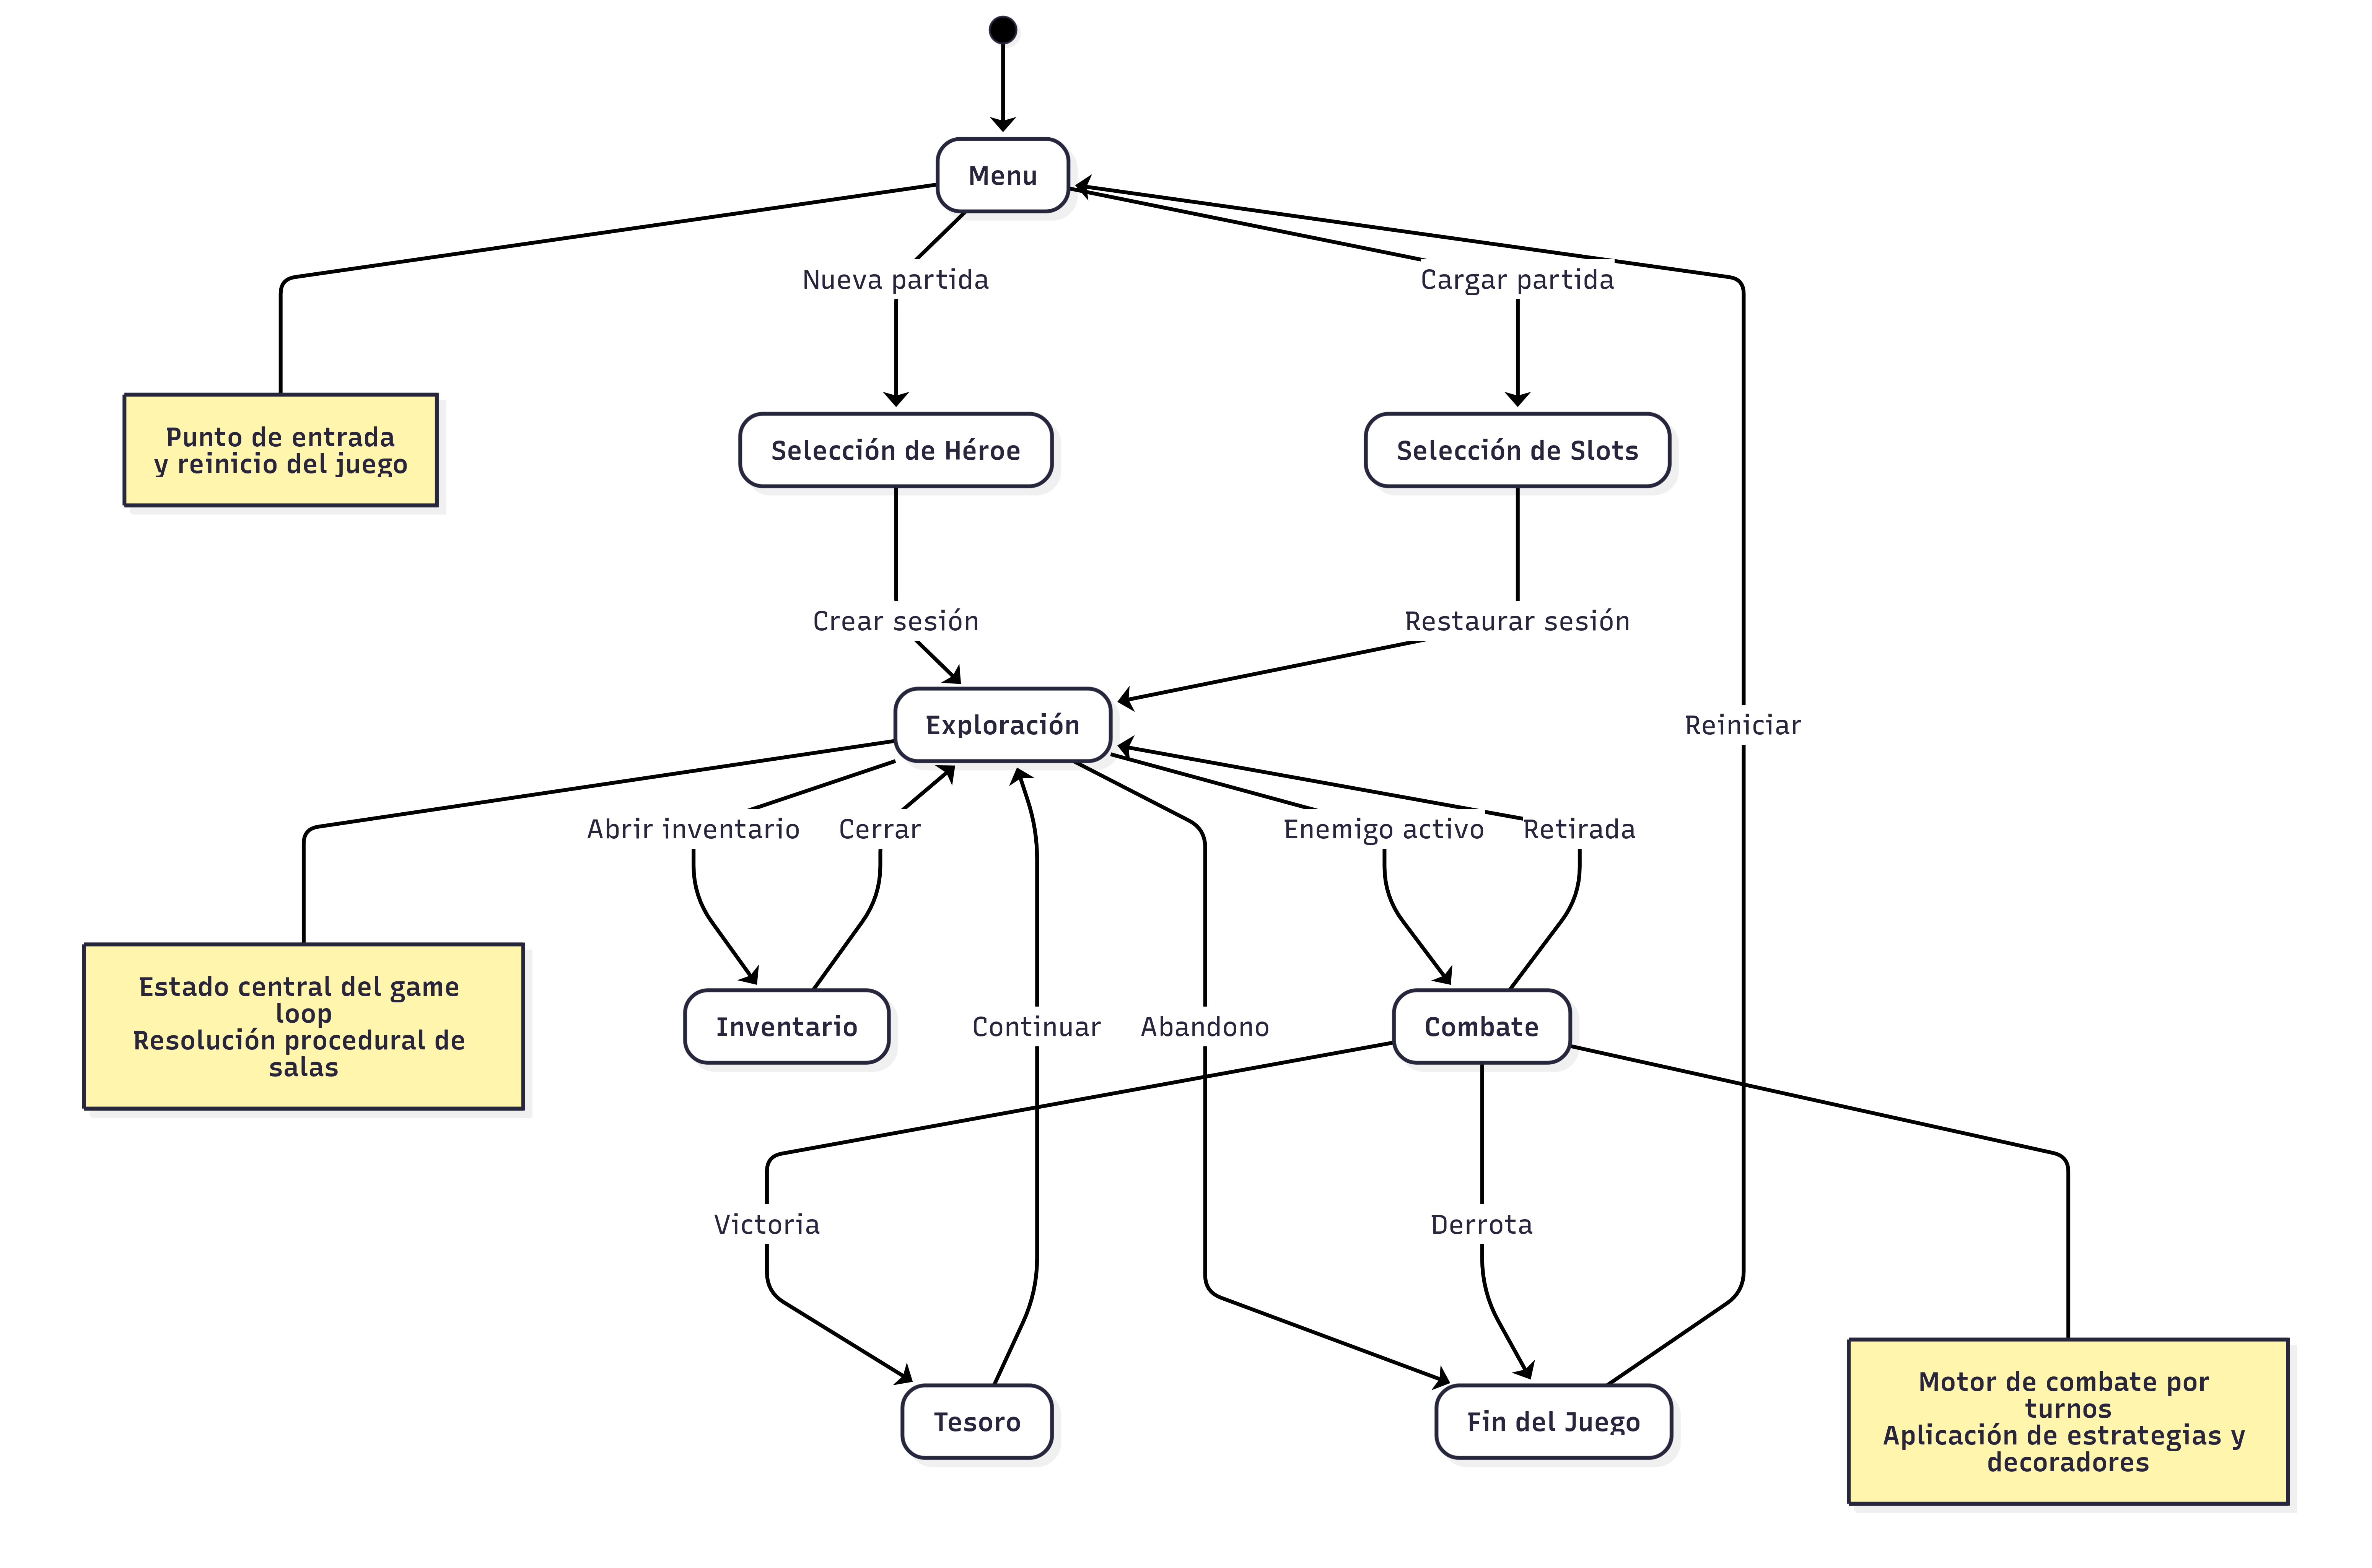
\includegraphics[width=0.9\textwidth]{Flujo de estados del sistema.png}
\caption{Diagrama de estados del sistema Eranthia. Transiciones: Menu → Heroe → Exploración → Combate → Tesoro → GameOver → Menu.}
\label{fig:flujo_estados}
\end{figure}

% =========================
% CASOS DE USO
% =========================

\section{Casos de Uso}

Los siguientes casos de uso describen el comportamiento observable del sistema desde la perspectiva del jugador, siguiendo la plantilla institucional con los campos: Nombre, Autor, Fecha, Descripción, Actores, Precondiciones, Flujo Normal, Flujo Alternativo y Poscondiciones. Cada caso de uso está respaldado por al menos un test de integración en la suite de 221 pruebas del proyecto.

\subsection{Diagrama General de Casos de Uso}

\begin{figure}[H]
\centering
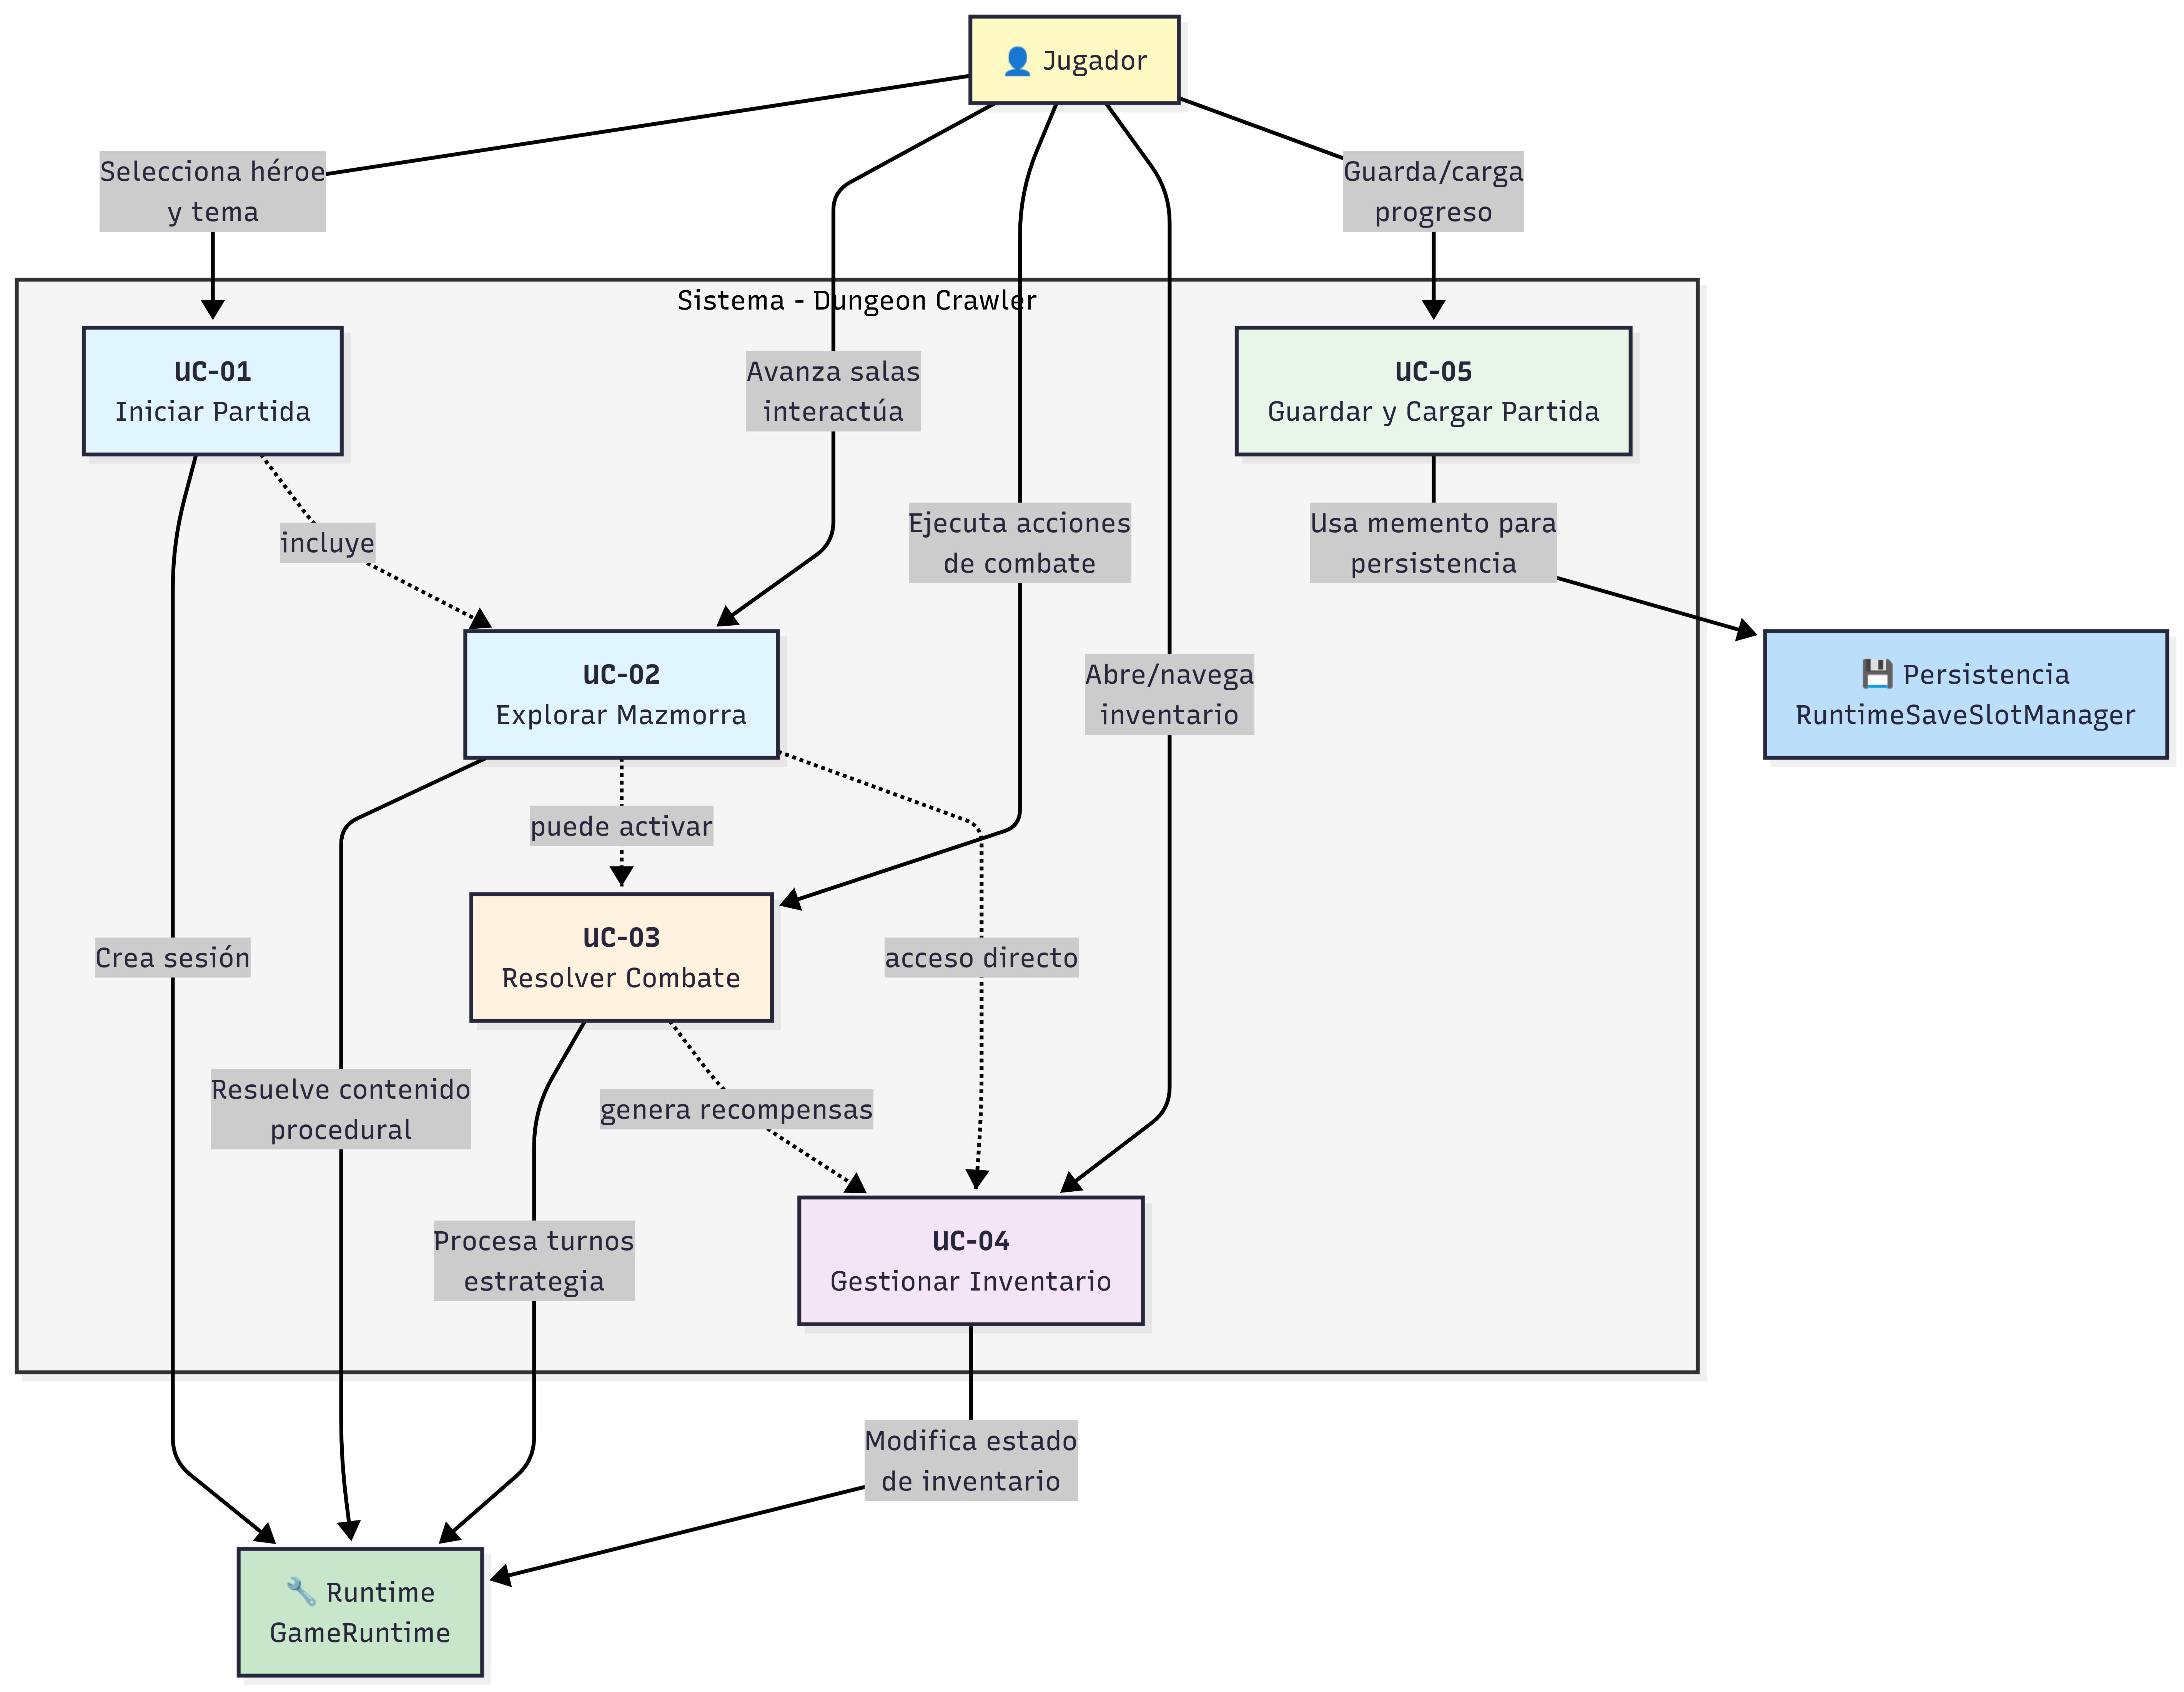
\includegraphics[width=0.85\textwidth]{Diagrama general casos de uso.png}
\caption{Diagrama UML general de casos de uso. Actor principal: Jugador. Casos de uso: CU-01 Iniciar partida, CU-02 Resolver combate, CU-03 Gestionar inventario, CU-04 Guardar/Cargar partida, CU-05 Explorar mazmorra.}
\label{fig:casos_uso}
\end{figure}

\subsection{Descripciones Detalladas de Casos de Uso}

% =========================
% CU-01: INICIAR NUEVA PARTIDA
% =========================

\subsection{CU-01: Iniciar Nueva Partida}

\begin{description}
    \item[Nombre:] CU-01: Iniciar Nueva Partida
    \item[Autor:] Andrés Felipe Martínez Henao
    \item[Fecha:] Mayo de 2026
    \item[Descripción:] Permite al jugador iniciar una nueva campaña seleccionando un héroe y un tema de mazmorra. El sistema crea una sesión de juego válida y transiciona al flujo de exploración.
    \item[Actores:] Jugador (actor principal); Sistema — GameRuntime, GameSessionFactory.
    \item[Precondiciones:] \hfill
        \begin{enumerate}[label=\arabic*.]
            \item El sistema se encuentra inicializado y en estado Menu.
            \item No existe una partida activa en memoria.
        \end{enumerate}
    \item[Flujo Normal:] \hfill
        \begin{enumerate}[label=\arabic*.]
            \item El jugador selecciona 'Nueva Partida' desde el menú principal.
            \item El sistema presenta las opciones de héroe (Guerrero, Mago, Arquero).
            \item El jugador selecciona un héroe.
            \item GameSessionFactory crea la sesión con el tema inicial (Poison).
            \item DungeonDirector genera la mazmorra procedural con seed aleatorio.
            \item GameStateContext transiciona al estado ExplorationState.
            \item El sistema renderiza la sala inicial con el héroe activo.
        \end{enumerate}
    \item[Flujo Alternativo:] \hfill
        \begin{enumerate}[label=FA-\arabic*:]
            \item El jugador cancela la selección → el sistema regresa al menú sin crear sesión.
            \item El payload de heroType es inválido → RuntimePayloadValidator rechaza el comando.
        \end{enumerate}
    \item[Poscondiciones:] \hfill
        \begin{enumerate}[label=\arabic*.]
            \item Existe una GameSession válida en estado Exploration.
            \item La mazmorra ha sido generada con seed persistido en el memento.
            \item Los observers de sesión están registrados y activos.
        \end{enumerate}
\end{description}

% =========================
% CU-02: RESOLVER COMBATE
% =========================

\subsection{CU-02: Resolver Combate por Turnos}

\begin{description}
    \item[Nombre:] CU-02: Resolver Combate por Turnos
    \item[Autor:] Andrés Felipe Martínez Henao
    \item[Fecha:] Mayo de 2026
    \item[Descripción:] El jugador se enfrenta a un enemigo activo en la sala. El sistema procesa las acciones del jugador y la respuesta de la IA enemiga por turnos hasta que el combate concluye en victoria, derrota o retirada.
    \item[Actores:] Jugador; Sistema — CombatFacade, CombatSystem, AIStrategy, CommandInvoker.
    \item[Precondiciones:] \hfill
        \begin{enumerate}[label=\arabic*.]
            \item Existe una GameSession activa en estado ExplorationState.
            \item La sala actual contiene un enemigo generado por DungeonThemeFactory.
            \item GameStateContext transiciona a CombatState al ingresar a la sala.
        \end{enumerate}
    \item[Flujo Normal:] \hfill
        \begin{enumerate}[label=\arabic*.]
            \item El sistema presenta la interfaz de combate con las acciones disponibles.
            \item El jugador selecciona una acción (Atacar, Defender, Habilidad, Ítem).
            \item GameRuntime valida la acción contra el estado activo (CombatState).
            \item CombatFacade delega la acción a CombatSystem vía CommandInvoker.
            \item AttackCommand calcula el daño aplicando CombatStatusDecoratorPipeline.
            \item CombatSystem.selectEnemyStrategy(hp\%) selecciona la IA según ratio de vida.
            \item El enemigo aplica su acción mediante AttackCommand registrado en el invoker.
            \item Si el enemigo llega a 0 HP → victoria; si el jugador → derrota; si no, regresa al paso 2.
        \end{enumerate}
    \item[Flujo Alternativo:] \hfill
        \begin{enumerate}[label=FA-\arabic*:]
            \item El jugador selecciona Retirada → CombatFacade.retreatAttempt() evalúa probabilidad y transiciona si es exitosa.
            \item El jugador usa un ítem → UseItemUseCase crea UseItemCommand y aplica efecto.
            \item Se aplica efecto de estado → CombatStatusDecoratorPipeline activa el decorator al inicio del turno.
        \end{enumerate}
    \item[Poscondiciones:] \hfill
        \begin{enumerate}[label=\arabic*.]
            \item Victoria: GameStateContext transiciona a TreasureState; se genera recompensa.
            \item Derrota: GameStateContext transiciona a GameOverState.
            \item El historial de CommandInvoker contiene todas las acciones ejecutadas.
        \end{enumerate}
\end{description}

% =========================
% CU-03: GESTIONAR INVENTARIO
% =========================

\subsection{CU-03: Gestionar Inventario Jerárquico}

\begin{description}
    \item[Nombre:] CU-03: Gestionar Inventario Jerárquico
    \item[Autor:] Andrés Felipe Martínez Henao
    \item[Fecha:] Mayo de 2026
    \item[Descripción:] El jugador accede al inventario durante la exploración, navega la estructura de contenedores anidados (patrón Composite) y puede usar o revisar sus ítems.
    \item[Actores:] Jugador; Sistema — Inventory, UseItemUseCase, ItemComponent, GameStateContext.
    \item[Precondiciones:] \hfill
        \begin{enumerate}[label=\arabic*.]
            \item Existe una GameSession activa en estado Exploration o Combat.
            \item El inventario contiene al menos un ítem disponible.
            \item GameStateContext permite la acción 'openInventory' desde el estado actual.
        \end{enumerate}
    \item[Flujo Normal:] \hfill
        \begin{enumerate}[label=\arabic*.]
            \item El jugador selecciona 'Inventario' desde la interfaz.
            \item GameStateContext transiciona a InventoryState.
            \item GamePresenter mapea Inventory.simpleItems() al GameViewModel para la UI.
            \item El jugador navega los contenedores (ContainerItem) e ítems simples (SimpleItem).
            \item El jugador selecciona un ítem y elige 'Usar'.
            \item UseItemUseCase.execute(itemId) crea UseItemCommand.
            \item Inventory.removeSimpleItemRecursive() consume el ítem de la jerarquía.
            \item El efecto del ítem se aplica al estado del héroe.
            \item El jugador cierra el inventario; GameStateContext regresa al estado anterior.
        \end{enumerate}
    \item[Flujo Alternativo:] \hfill
        \begin{enumerate}[label=FA-\arabic*:]
            \item El ítem no existe en la jerarquía → UseItemUseCase devuelve error sin modificar la sesión.
            \item El jugador solo revisa sin usar → el sistema muestra la estructura sin mutación.
            \item El inventario está vacío → el sistema muestra mensaje 'Sin ítems disponibles'.
        \end{enumerate}
    \item[Poscondiciones:] \hfill
        \begin{enumerate}[label=\arabic*.]
            \item El ítem usado ha sido eliminado de la jerarquía Composite.
            \item Las estadísticas del héroe reflejan el efecto del ítem.
            \item El árbol Composite mantiene su integridad jerárquica.
        \end{enumerate}
\end{description}

% =========================
% CU-04: GUARDAR Y CARGAR
% =========================

\subsection{CU-04: Guardar y Cargar Partida}

\begin{description}
    \item[Nombre:] CU-04: Guardar y Cargar Partida
    \item[Autor:] Andrés Felipe Martínez Henao
    \item[Fecha:] Mayo de 2026
    \item[Descripción:] El jugador persiste el estado completo de la sesión en un slot numerado, o restaura una partida previa. El patrón Memento garantiza snapshots atómicos con validación de versión de esquema (schemaVersion 1.0).
    \item[Actores:] Jugador; Sistema — RuntimeSaveSlotManager, SaveGameUseCase, LoadGameUseCase, GameCaretaker, GameSessionMementoMapper.
    \item[Precondiciones:] \hfill
        \begin{description}
            \item[Guardar:] existe una GameSession activa en estado Exploration (no en combate activo).
            \item[Cargar:] existe al menos un slot guardado en el sistema de archivos (game-saves/).
        \end{description}
    \item[Flujo Normal:] \hfill
        \begin{description}
            \item[GUARDAR:] \hfill
                \begin{enumerate}[label=\arabic*.]
                    \item El jugador indica el slot destino (1-3).
                    \item RuntimeSaveSlotManager invoca SaveGameUseCase.
                    \item GameSessionMementoMapper.toMemento() serializa la sesión con schemaVersion='1.0'.
                    \item GameCaretaker persiste el archivo en game-saves/Slot\_n.save.
                \end{enumerate}
            \item[CARGAR:] \hfill
                \begin{enumerate}[label=\arabic*.]
                    \item El jugador selecciona el slot a restaurar.
                    \item GameCaretaker.cargarDesdeDisco() lee el archivo.
                    \item restoreStrict() valida schemaVersion y restaura el estado completo.
                    \item GameStateContext transiciona al estado guardado.
                \end{enumerate}
        \end{description}
    \item[Flujo Alternativo:] \hfill
        \begin{enumerate}[label=FA-\arabic*:]
            \item Slot vacío al cargar → SaveSlotNotFoundException; sesión sin cambios.
            \item Archivo corrompido o versión incompatible → SaveDataCorruptionException.
            \item Intento de guardar durante combate → SaveGameUseCase rechaza la operación.
            \item Fallo inesperado → UseCaseTransactionSupport restaura el snapshot previo (rollback).
        \end{enumerate}
    \item[Poscondiciones:] \hfill
        \begin{description}
            \item[Guardar:] existe el archivo Slot\_n.save con datos íntegros.
            \item[Cargar:] la GameSession refleja exactamente el estado del momento del guardado.
        \end{description}
\end{description}

% =========================
% CU-05: EXPLORAR MAZMORRA
% =========================

\subsection{CU-05: Explorar Mazmorra y Progresar Campaña}

\begin{description}
    \item[Nombre:] CU-05: Explorar Mazmorra y Progresar Campaña
    \item[Autor:] Andrés Felipe Martínez Henao
    \item[Fecha:] Mayo de 2026
    \item[Descripción:] El jugador avanza por las salas de la mazmorra. El sistema resuelve el contenido procedural de cada sala y gestiona la progresión de campaña entre biomas (Poison → Ice → Fire → Dark).
    \item[Actores:] Jugador; Sistema — GameRuntime, ProceduralDungeonGenerator, DungeonThemeFactory, CampaignSessionCoordinator, GameStateContext.
    \item[Precondiciones:] \hfill
        \begin{enumerate}[label=\arabic*.]
            \item Existe una GameSession activa en estado ExplorationState.
            \item La mazmorra ha sido generada por DungeonDirector.buildForTheme(tema, seed).
            \item El jugador tiene HP mayor a 0.
        \end{enumerate}
    \item[Flujo Normal:] \hfill
        \begin{enumerate}[label=\arabic*.]
            \item El sistema presenta la sala actual con sus opciones de avance.
            \item El jugador elige avanzar a la siguiente sala.
            \item El sistema resuelve el contenido de la sala:
                \begin{enumerate}[label=\alph*)]
                    \item Sala con enemigo → CombatState (CU-02).
                    \item Sala de tesoro → recompensa temática de DungeonThemeFactory.
                    \item Sala vacía → el jugador continúa sin evento.
                \end{enumerate}
            \item Al completar todas las salas, CampaignSessionCoordinator avanza al siguiente bioma.
            \item DungeonDirector genera la nueva mazmorra para el nuevo tema.
            \item EventManager notifica el evento de progresión a los observers registrados.
        \end{enumerate}
    \item[Flujo Alternativo:] \hfill
        \begin{enumerate}[label=FA-\arabic*:]
            \item El jugador derrota al jefe → flujo de victoria activa la transición de bioma.
            \item El jugador abre el inventario → CU-03; al cerrar regresa a ExplorationState.
            \item Final de campaña (Dark completado) → pantalla de victoria y regreso al menú.
            \item HP llega a 0 durante exploración → GameStateContext transiciona a GameOverState.
        \end{enumerate}
    \item[Poscondiciones:] \hfill
        \begin{enumerate}[label=\arabic*.]
            \item La sala visitada está marcada como explorada en el estado de la mazmorra.
            \item Si hubo cambio de bioma: la nueva mazmorra está generada y persistida.
            \item Los eventos emitidos quedaron registrados en SessionEventCounterObserver.
        \end{enumerate}
\end{description}

% =========================
% PROTOTIPADO
% =========================

\section{Prototipado de Interfaz}

El prototipado de la interfaz de usuario de Eranthia fue desarrollado utilizando Google Stitch. El prototipo sirvió como referencia visual durante el desarrollo; las modificaciones surgidas en la implementación real se registran en esta sección.

\subsection{Pantallas Prototipadas}

\begin{table}[H]
\centering
\caption{Pantallas prototipadas y cambios respecto al prototipo original}
\begin{tabular}{p{2cm}p{3.5cm}p{4.5cm}}
\toprule
\textbf{Pantalla} & \textbf{Descripción} & \textbf{Cambios respecto al prototipo} \\
\midrule
Menú principal & Pantalla de inicio con opciones Nueva Partida, Cargar Partida y Salir. & Se simplificó la navegación; se eliminó la selección de dificultad global. \\

Selección de héroe & Pantalla de selección entre Guerrero, Mago y Arquero con descripción de stats. & Se consolidó la selección con la elección de tema de campaña. \\

Exploración & Vista en primera persona de los pasillos de la mazmorra con indicadores de sala y opciones de avance. & Se añadió el panel lateral de stats del héroe en tiempo real. \\

Combate & Interfaz de combate por turnos con panel de acciones, barra de HP y log de eventos. & Se implementó jerarquía de botones de tres niveles: acciones primarias, estilos y situacionales. \\

Inventario & Panel de inventario jerárquico con árbol de contenedores e ítems simples. & Se conservó la estructura Composite visible al jugador mediante lista plana con indicadores de anidamiento. \\
\bottomrule
\end{tabular}
\caption*{\textit{Nota.} Elaboración propia. El prototipo original está disponible en: https://stitch.withgoogle.com/projects/4618622630132809698}
\end{table}

Las interfaces son temáticas, por lo cual cada mazmorra tiene un color distintivo que facilita la identificación visual del bioma actual en la campaña.

\subsection{Capturas del Prototipo}

La siguiente colección de imágenes presenta las pantallas principales del juego tal como fueron prototipadas en Google Stitch y su implementación final en la interfaz de usuario.

\begin{figure}[H]
\centering
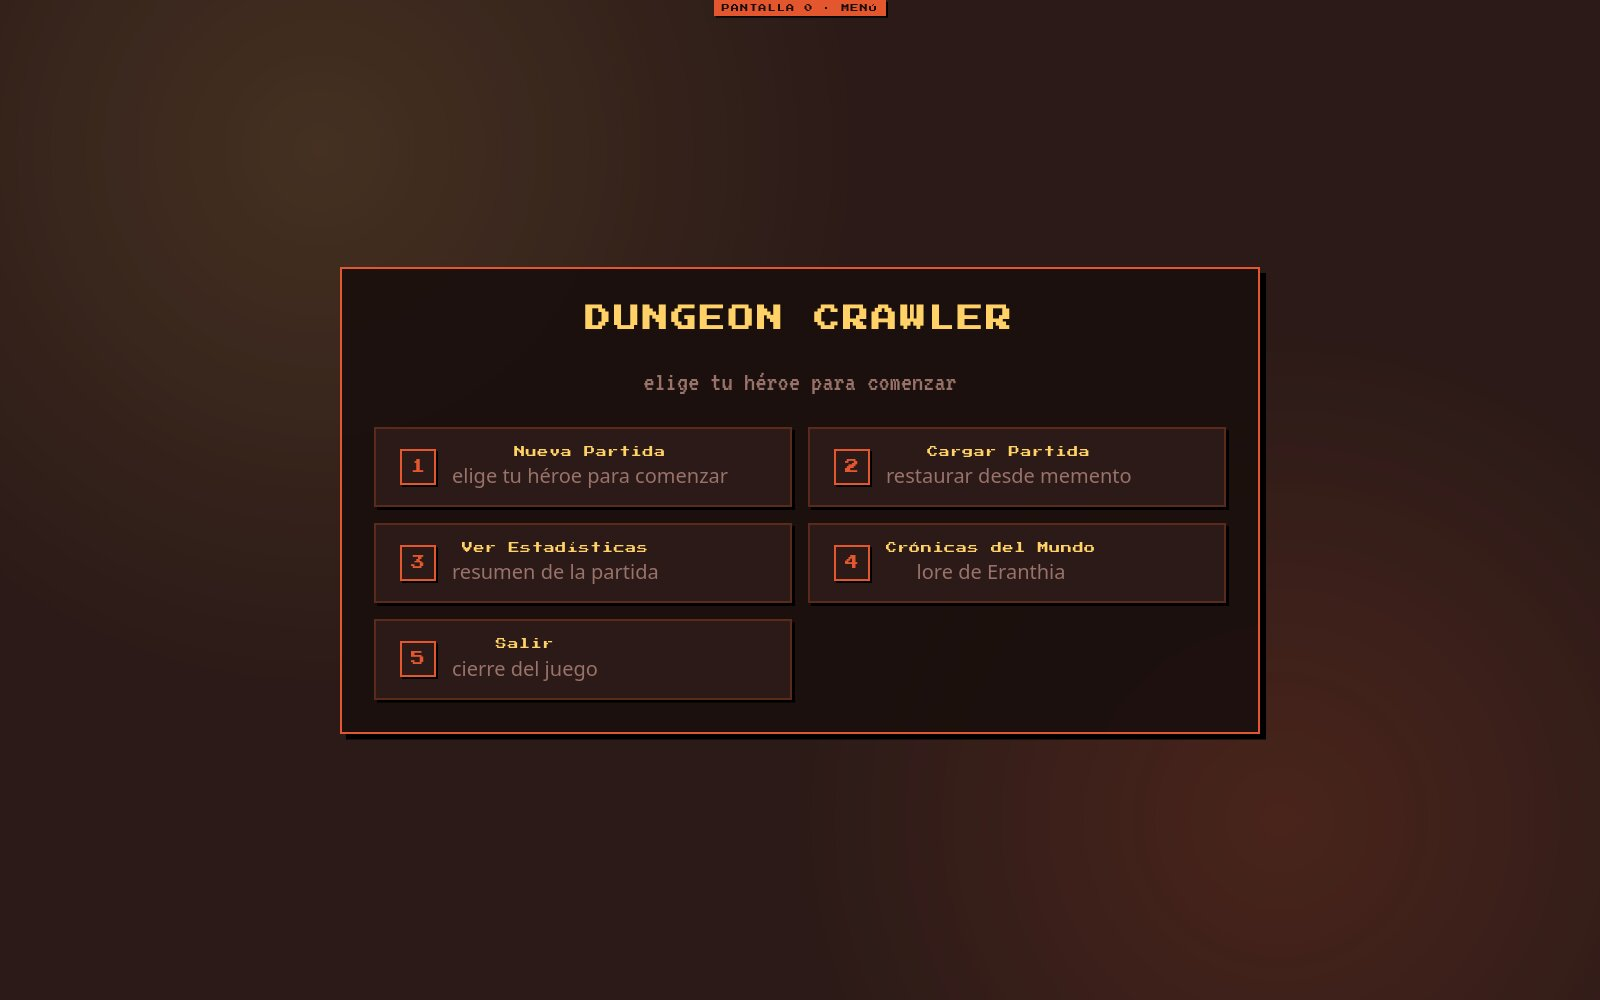
\includegraphics[width=0.6\textwidth]{Menu_Principal.jpg}
\caption{Pantalla del Menú Principal con opciones Nueva Partida, Cargar Partida y Salir.}
\label{fig:menu_principal}
\end{figure}

\begin{figure}[H]
\centering
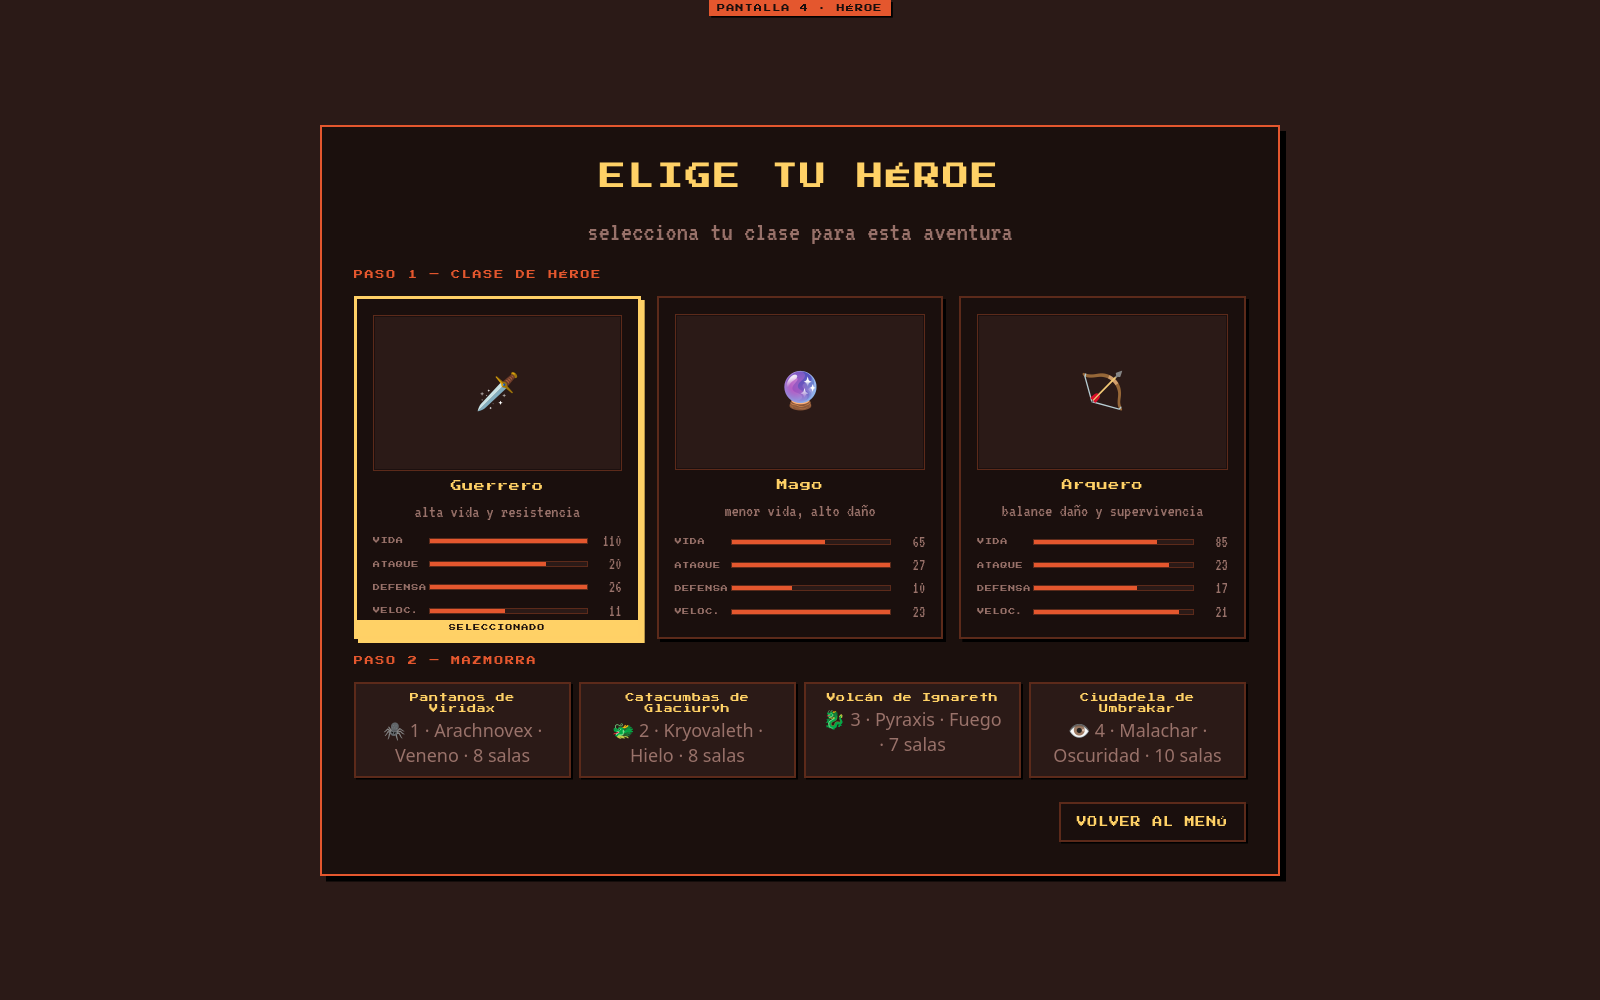
\includegraphics[width=0.7\textwidth]{Seleccion de Heroe y Mazmorra.png}
\caption{Pantalla de Selección de Héroe y Tema de Campaña. El jugador elige entre Guerrero, Mago o Arquero y confirma el tema inicial (Poison).}
\label{fig:seleccion_heroe}
\end{figure}

\begin{figure}[H]
\centering
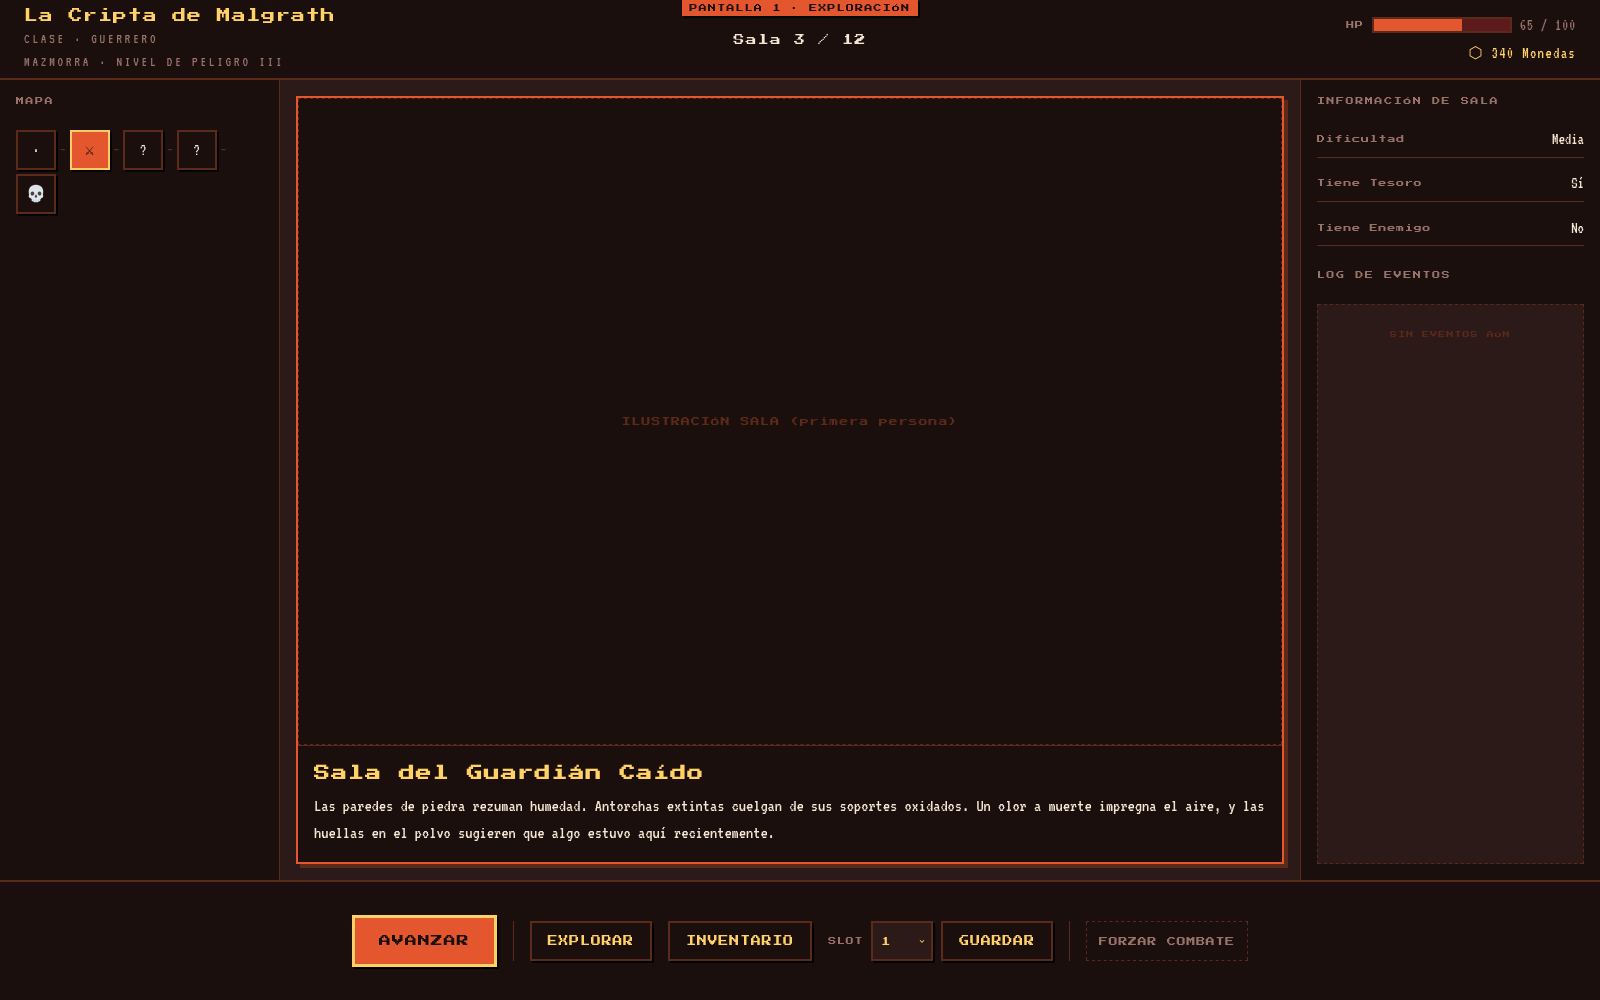
\includegraphics[width=0.75\textwidth]{Exploracion.png}
\caption{Interfaz de Exploración de Mazmorra. Visualización de la sala actual con indicadores de progresión, panel de estadísticas del héroe y opciones de avance.}
\label{fig:exploracion}
\end{figure}

\begin{figure}[H]
\centering
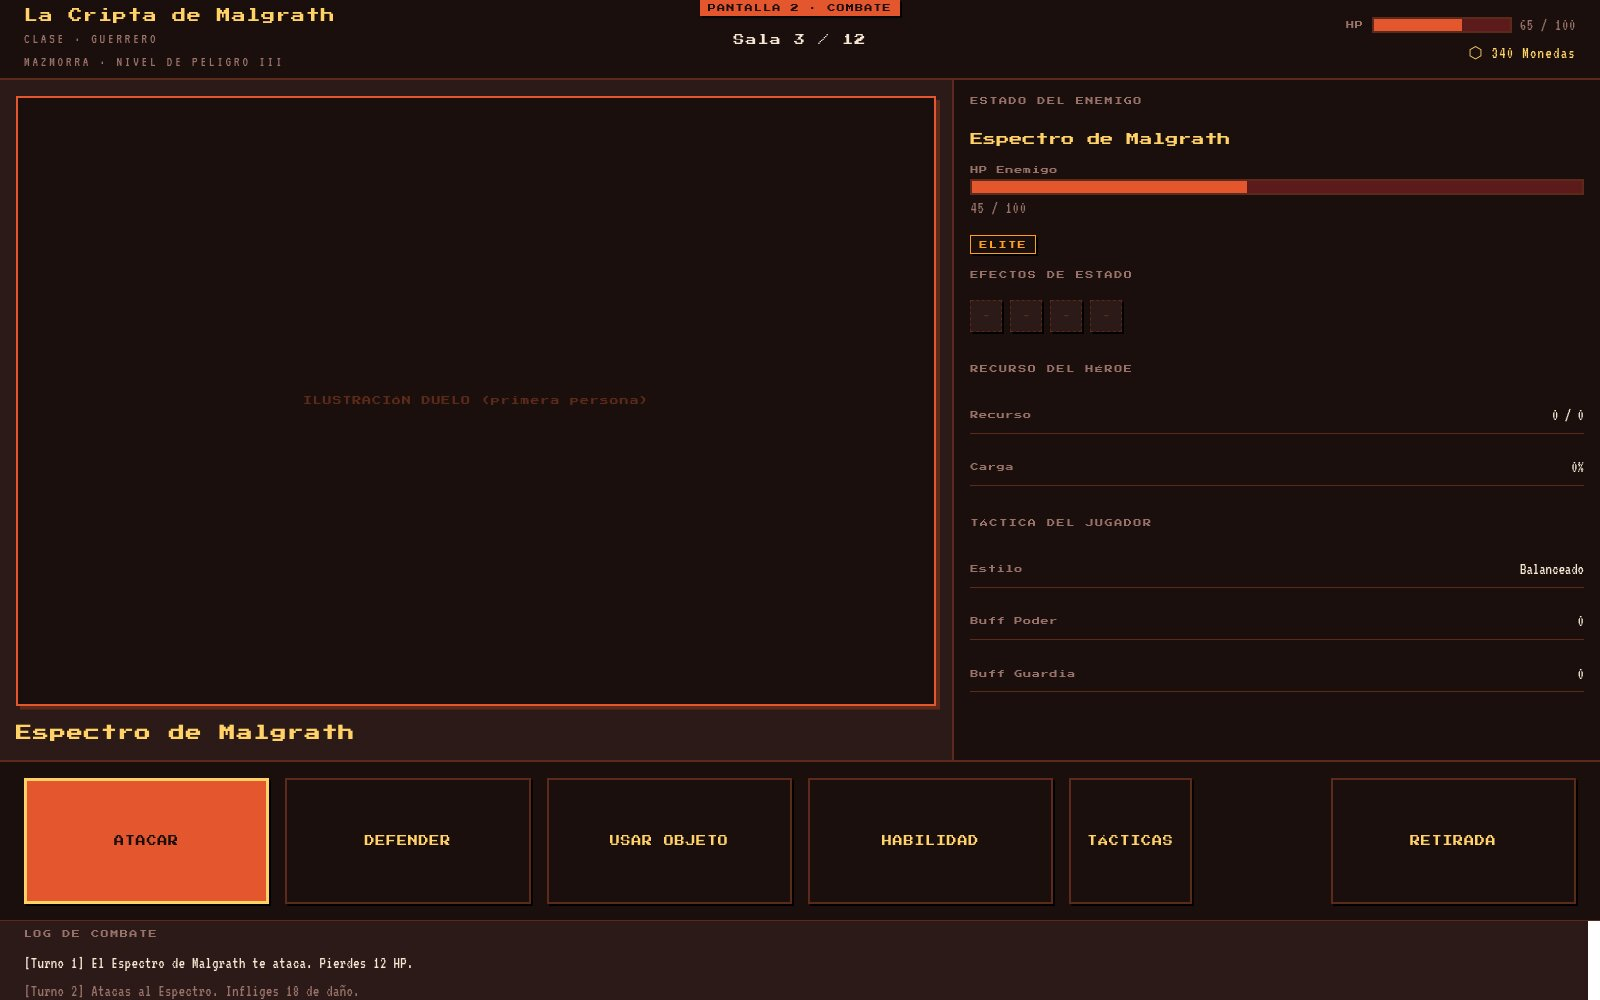
\includegraphics[width=0.7\textwidth]{Combate.jpg}
\caption{Interfaz de Combate por Turnos. Panel de acciones (Atacar, Defender, Habilidad, Ítem), barras de HP enemigo y jugador, y log de eventos del combate.}
\label{fig:combate}
\end{figure}

\begin{figure}[H]
\centering
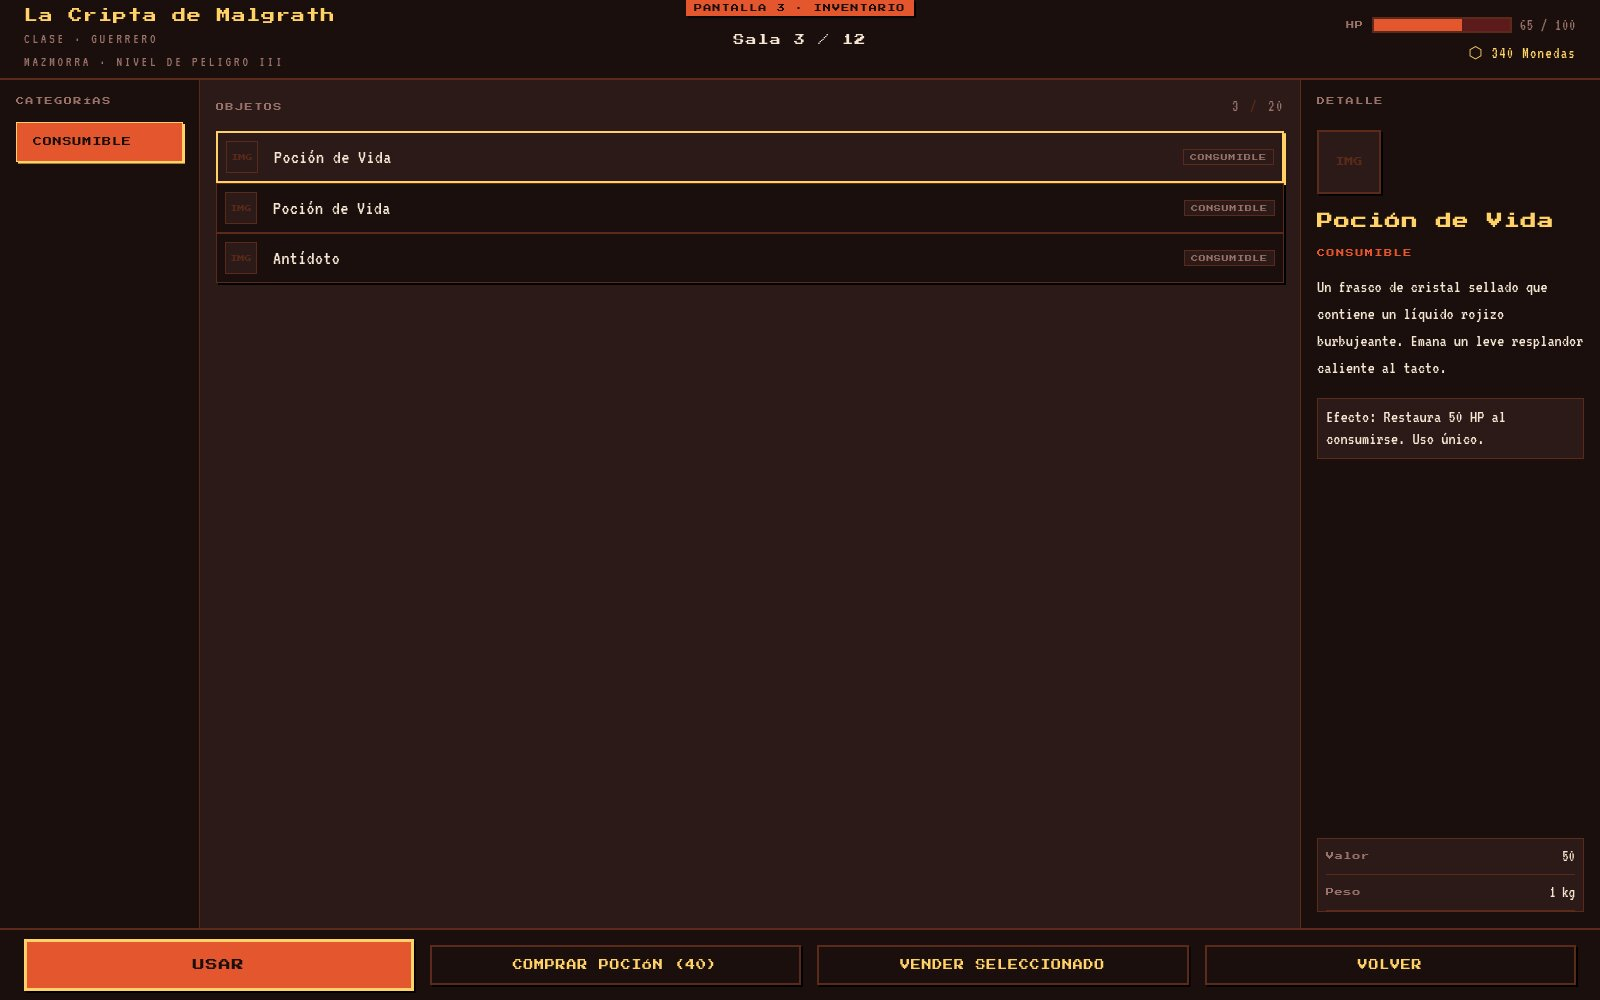
\includegraphics[width=0.65\textwidth]{Inventario.jpg}
\caption{Pantalla de Inventario Jerárquico. Visualización de contenedores e ítems simples con indicadores de anidamiento. Permite revisar y usar objetos durante la partida.}
\label{fig:inventario}
\end{figure}

\begin{figure}[H]
\centering
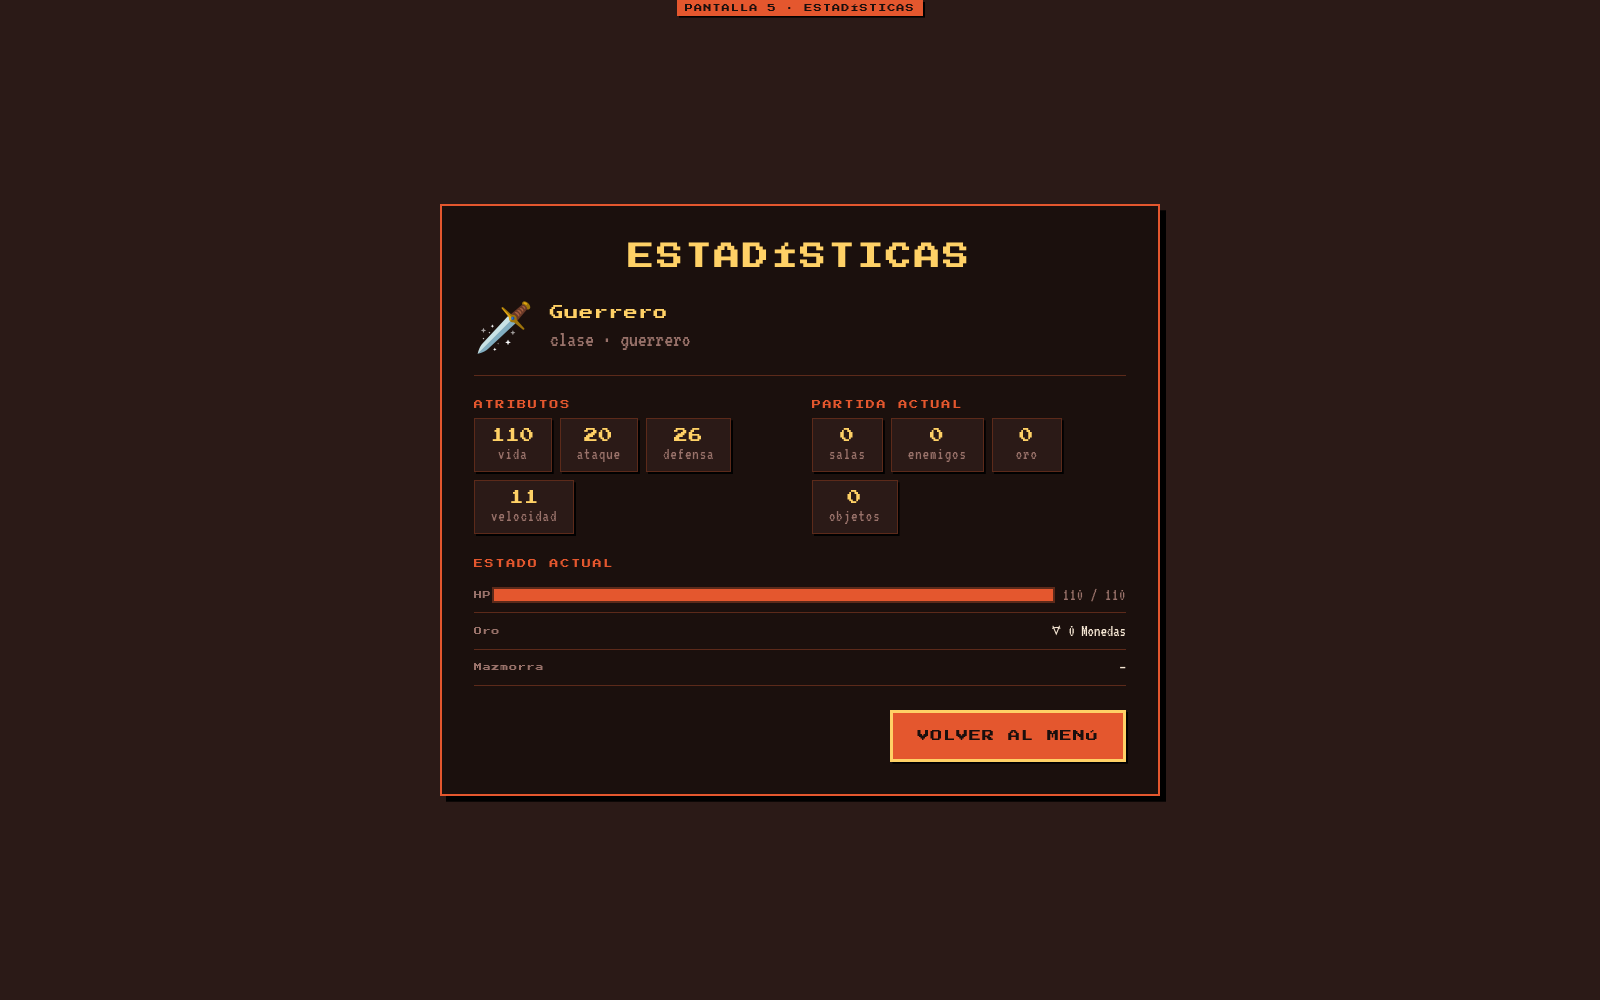
\includegraphics[width=0.65\textwidth]{Ventana de estadisticas.png}
\caption{Pantalla de Estadísticas del Héroe. Resumen de atributos (HP, Ataque, Defensa, Experiencia) y progresión de la campaña por biomas.}
\label{fig:estadisticas}
\end{figure}

\begin{figure}[H]
\centering
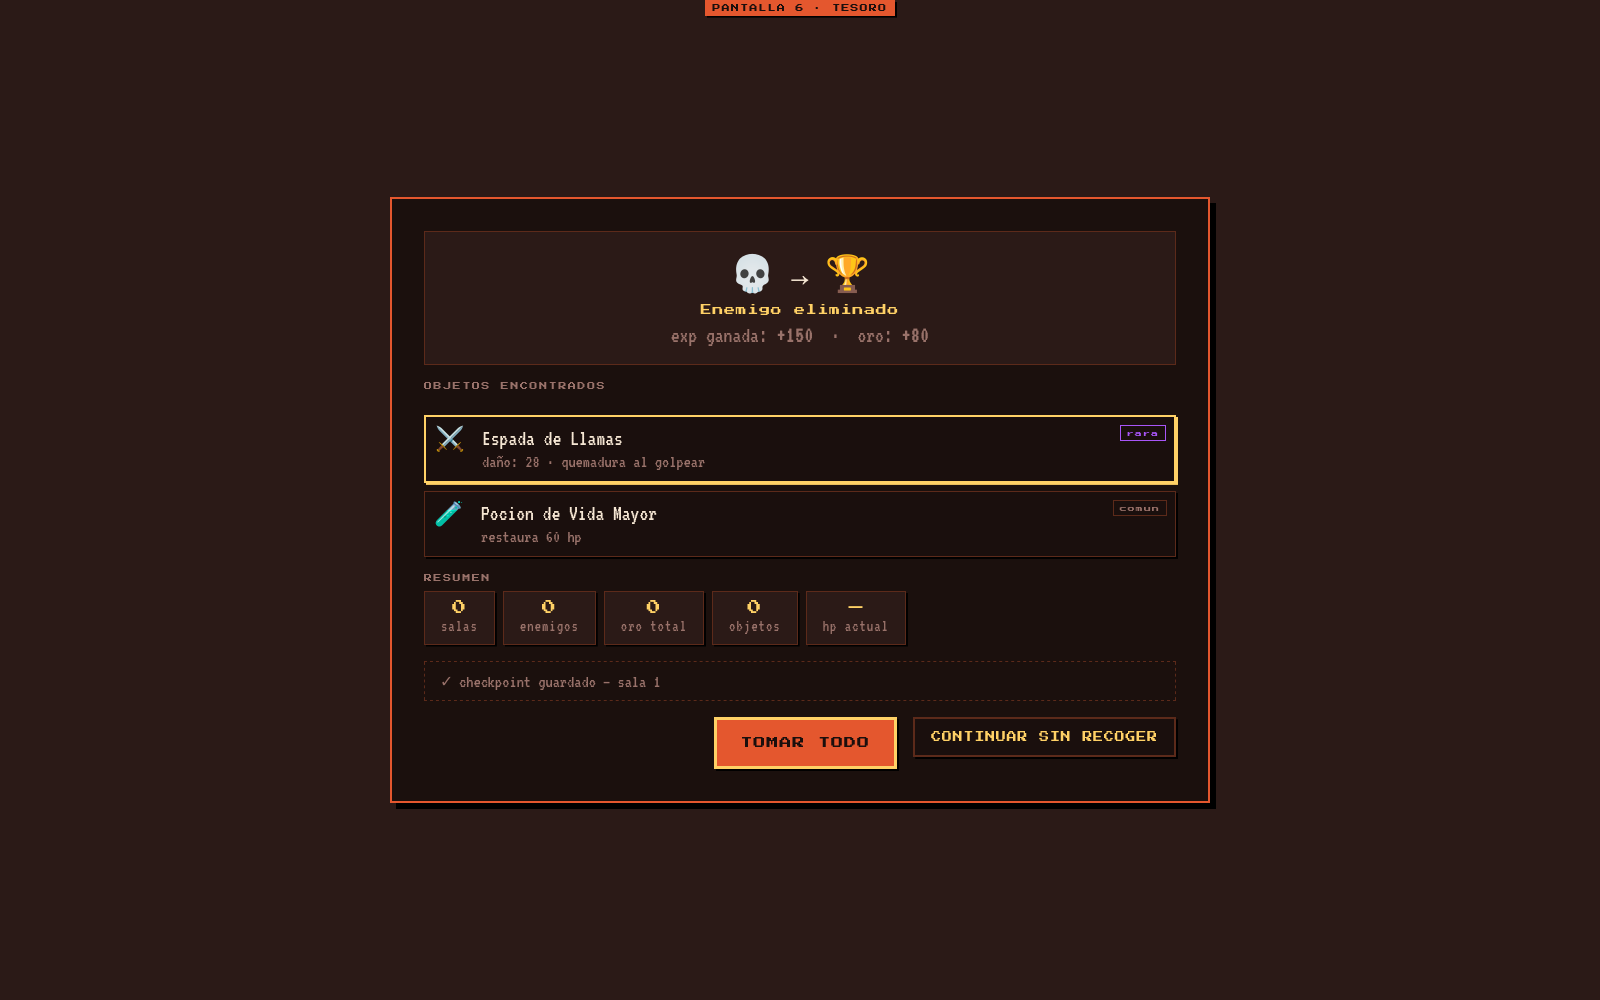
\includegraphics[width=0.65\textwidth]{Ventana de victoria.png}
\caption{Pantalla de Victoria. Se muestra al completar un combate exitosamente con recompensas obtenidas (oro, experiencia, ítems).}
\label{fig:victoria}
\end{figure}

\begin{figure}[H]
\centering
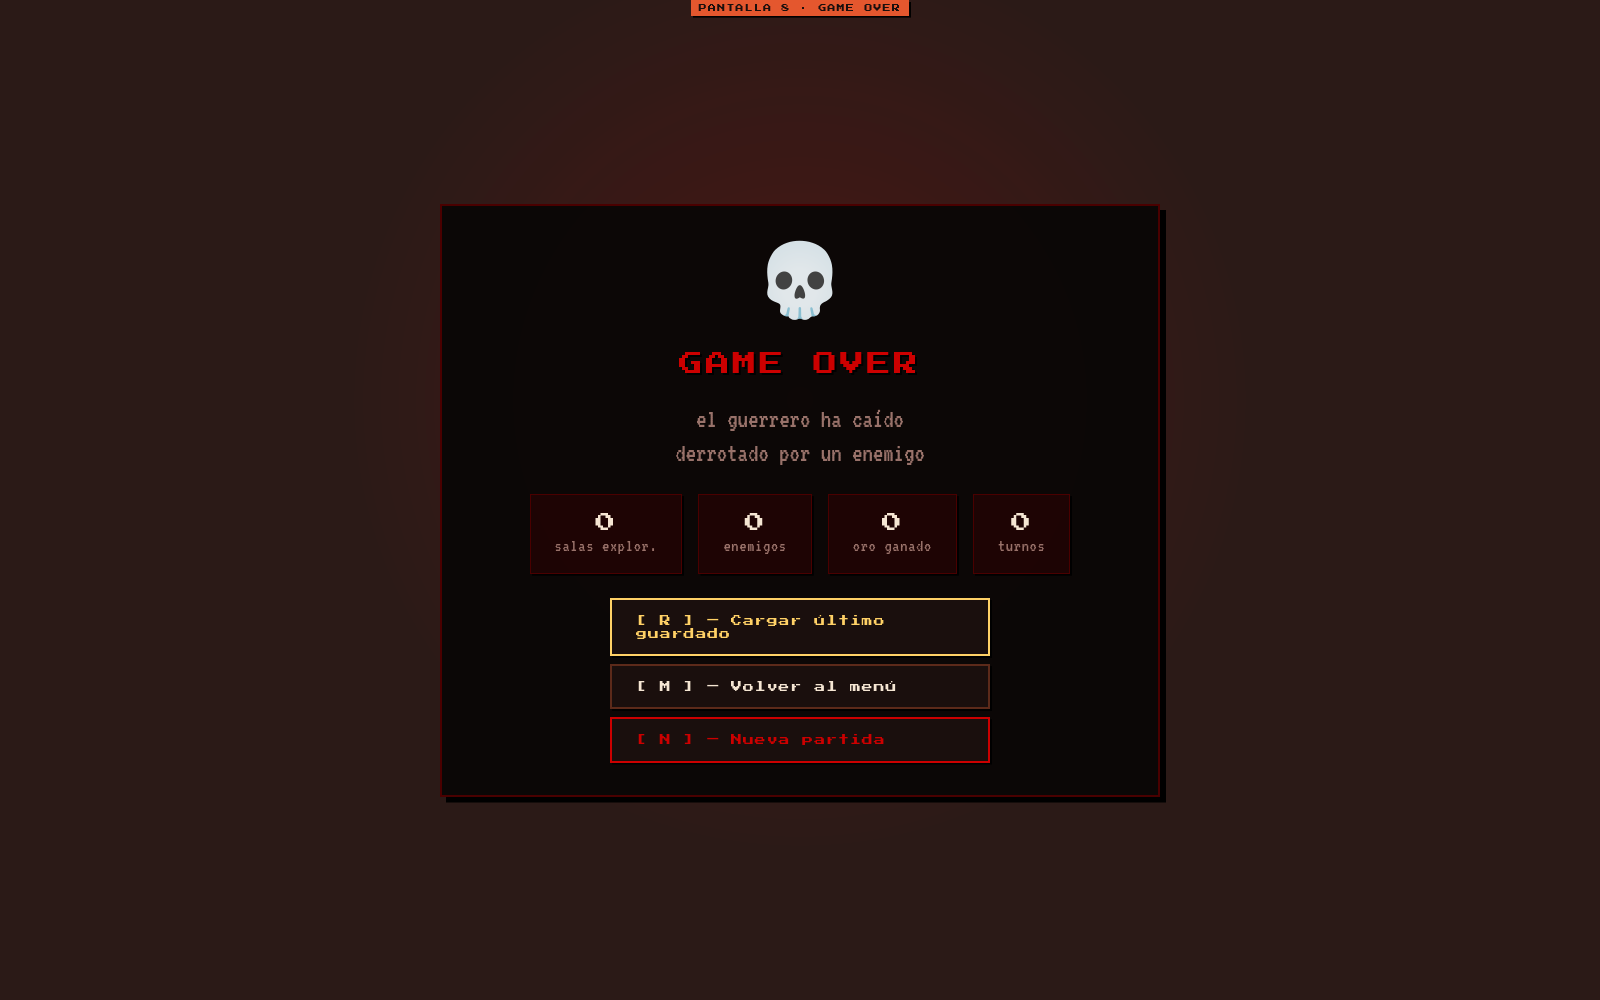
\includegraphics[width=0.65\textwidth]{Ventana de derrota.png}
\caption{Pantalla de Derrota o Game Over. Se muestra cuando el héroe llega a 0 HP. Ofrece opciones para reintentar o volver al menú principal.}
\label{fig:derrota}
\end{figure}

\begin{figure}[H]
\centering
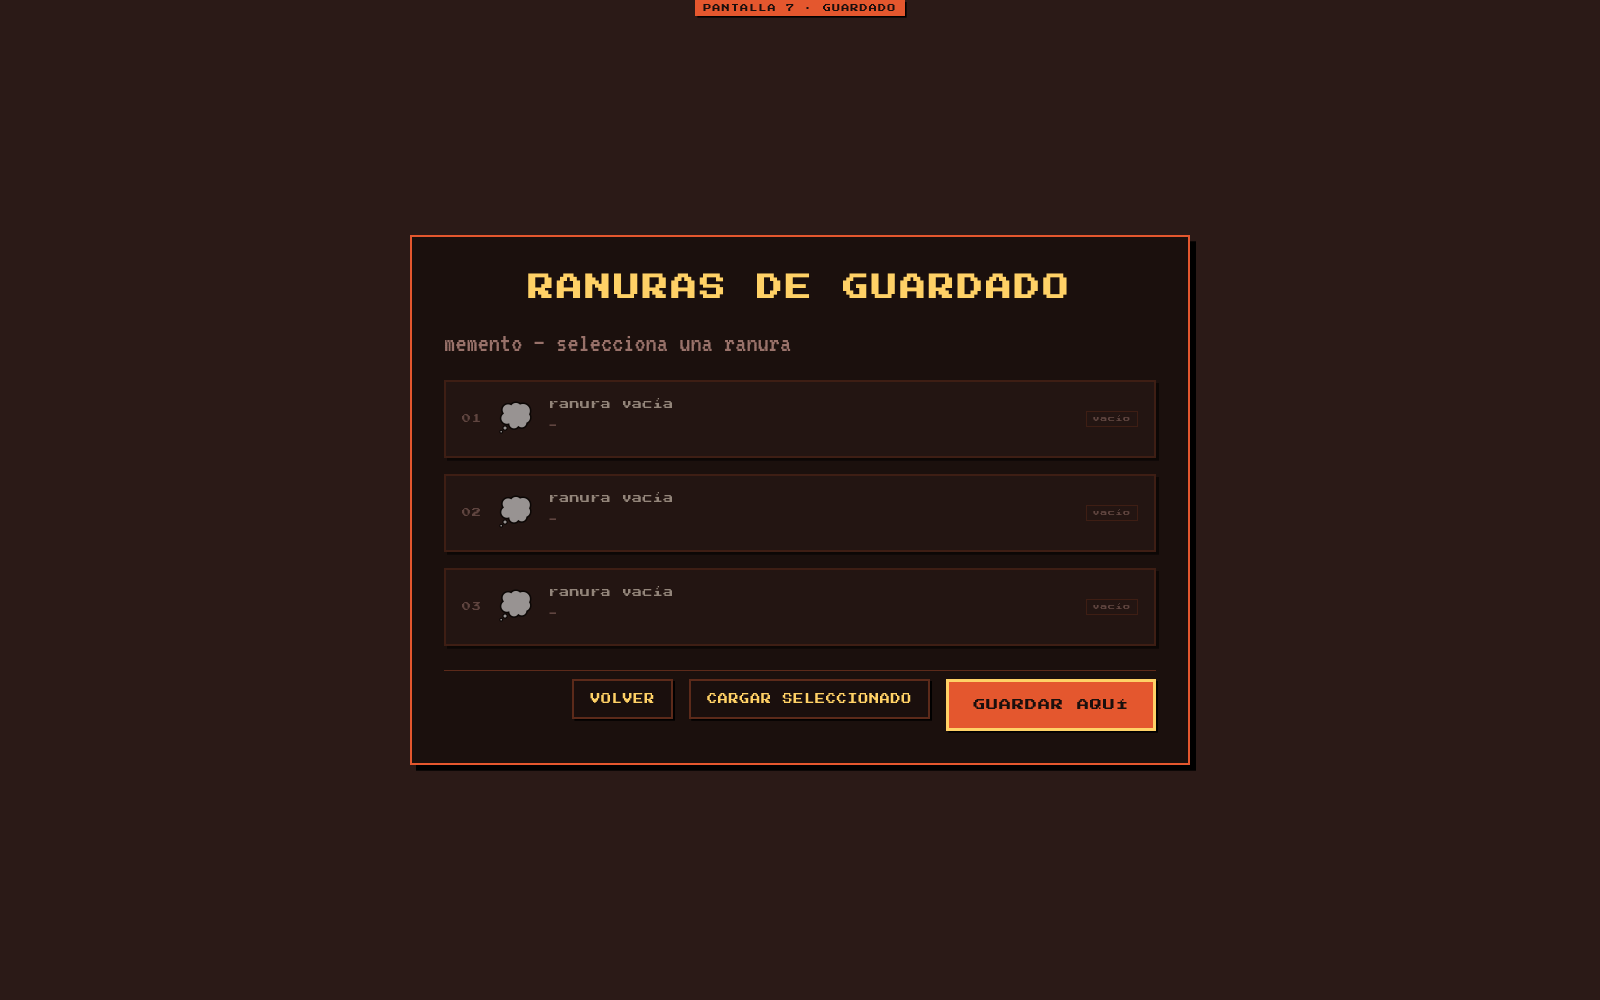
\includegraphics[width=0.65\textwidth]{Venta de Slots.png}
\caption{Interfaz de Gestión de Slots de Guardado. Permite al jugador guardar partidas en tres slots independientes o cargar una partida previa con información de fecha y progresión.}
\label{fig:slots}
\end{figure}

% =========================
% POO
% =========================

\section{Pilares de la Programación Orientada a Objetos}

La programación orientada a objetos (POO) se fundamenta en cuatro pilares: encapsulamiento, herencia, polimorfismo y abstracción \cite{cairo2022}. A continuación se evidencia la presencia de cada pilar en la arquitectura de Eranthia con referencias directas al código fuente.

\subsection{Encapsulamiento}

El encapsulamiento protege el estado interno de un objeto y expone solo la interfaz necesaria para interactuar con él. En Eranthia, este principio se aplica de forma sistemática en toda la capa de dominio y aplicación.

La clase GameSession concentra el estado completo de la sesión de juego (héroe, mazmorra, combate, inventario, flujo de pantallas) y lo expone únicamente a través de métodos públicos controlados. Ninguna capa externa accede directamente a sus atributos privados. El método assertActionAllowed(accion) encapsula la lógica de validación delegando en GameStateContext, de modo que el consumidor (GameRuntime) no conoce los detalles de la política de estados.

El patrón Memento refuerza el encapsulamiento al separar la creación del snapshot (GameSessionMementoMapper.toMemento()) del almacenamiento físico (GameCaretaker). El objeto GameMemento es inmutable: expone solo getters y no permite modificación externa de su estado serializado.

RuntimePayloadValidator encapsula todas las reglas de validación estructural de comandos UI, evitando que GameRuntime deba conocer los criterios de validación de cada tipo de payload. Esto reduce el acoplamiento y facilita la extensión de reglas sin modificar el orquestador.

\subsection{Herencia}

La herencia permite que una clase hija reutilice y extienda el comportamiento de una clase padre, estableciendo jerarquías de tipo. Eranthia emplea herencia de forma deliberada en sus jerarquías de dominio y patrones estructurales.

La jerarquía de personajes parte de la clase abstracta Personaje, que define atributos comunes (nombre, HP, ataque, defensa) y comportamientos base como recibirDanio() y estaVivo(). Las clases concretas Guerrero, Mago, Arquero, EnemigoBasico, Orco y Dragon extienden esta clase añadiendo o sobreescribiendo comportamientos específicos (stats diferenciados, habilidades exclusivas de clase).

El patrón Decorator construye su jerarquía sobre CharacterDecorator, clase abstracta que extiende Personaje y envuelve una instancia del mismo tipo. Las clases concretas PoisonEffect, BurnEffect, StunEffect, StrengthEffect y GuardEffect heredan de CharacterDecorator, permitiendo el anidamiento dinámico de efectos sin duplicar lógica de personaje base.

En el patrón Command, la interfaz Command es implementada por todas las acciones concretas (AttackCommand, DefendCommand, UseItemCommand, SkillCommand, LevelUpCommand), garantizando que CommandInvoker pueda ejecutar cualquier acción sin conocer su tipo concreto.

\subsection{Polimorfismo}

El polimorfismo permite tratar objetos de tipos distintos a través de una interfaz común, resolviendo el comportamiento correcto en tiempo de ejecución. Es el pilar que hace posible la intercambiabilidad de implementaciones en Eranthia.

CombatSystem invoca selectEnemyStrategy(hp\%) y obtiene en cada llamada una instancia distinta de AIStrategy (AggressiveStrategy, DefensiveStrategy, IntelligentStrategy o RandomStrategy) dependiendo del ratio de vida del enemigo. El sistema de combate no conoce ni le importa cuál estrategia concreta se ejecuta: invoca decidirAccion() y obtiene un Command válido.

DungeonThemeFactory permite que GameSessionFactory resuelva en tiempo de ejecución la factory concreta (FireThemeFactory, IceThemeFactory, PoisonThemeFactory, DarkThemeFactory) mediante el mismo tipo de referencia. Cada factory crea enemigos y loot con resistencias y propiedades distintas sin que el orquestador lo sepa.

El árbol Composite de Inventory opera íntegramente sobre el tipo abstracto ItemComponent. Los métodos getValorTotal(), getPesoTotal() y deepCopy() se resuelven polimórficamente: en SimpleItem retornan los valores del ítem hoja; en ContainerItem suman recursivamente los valores de todos los hijos.

\subsection{Abstracción}

La abstracción consiste en modelar entidades del dominio ocultando los detalles de implementación irrelevantes y exponiendo solo las operaciones esenciales. En Eranthia, la abstracción se materializa en interfaces, clases abstractas y fachadas.

La interfaz AIStrategy abstrae el concepto de 'decisión enemiga' en un único método decidirAccion(). Cualquier algoritmo de IA puede incorporarse al sistema implementando esta interfaz, sin requerir cambios en CombatSystem. Lo mismo aplica a GameObserver, que abstrae el concepto de 'escucha de eventos' en onEvent(GameEvent).

CombatFacade abstrae toda la complejidad del subsistema de combate (Combat, CombatSystem, TurnManager, CombatStatusDecoratorPipeline) detrás de una API limpia de más de treinta métodos públicos bien definidos. GameSession.combat() retorna la fachada y los casos de uso operan exclusivamente a través de ella, sin conocer los subsistemas internos.

GamePresenter abstrae el mapeo entre el estado interno de la sesión y el GameViewModel consumido por la UI. La interfaz web y la interfaz de consola no conocen la estructura interna de GameSession: reciben únicamente el modelo de vista serializado como JSON.

% =========================
% SOLID
% =========================

\section{Principios SOLID}

Los principios SOLID son un conjunto de cinco directrices de diseño orientado a objetos formuladas por Robert C. Martin que buscan producir sistemas más comprensibles, flexibles y mantenibles \cite{martin2003}. A continuación se analiza la aplicación de cada principio en la arquitectura de Eranthia.

\subsection{Single Responsibility Principle}

El principio de responsabilidad única establece que una clase debe tener una sola razón para cambiar. En Eranthia, el cumplimiento de este principio fue el resultado directo del ciclo de auditoría: la clase GameRuntime fue identificada como un 'God Object' y refactorizada en tres colaboradores de responsabilidad única.

RuntimePayloadValidator tiene una sola responsabilidad: validar la estructura y semántica de los payloads de comandos provenientes de la UI antes de que muten la sesión. RuntimeSaveSlotManager tiene una sola responsabilidad: gestionar la resolución de slots y delegar en SaveGameUseCase/LoadGameUseCase. CampaignSessionCoordinator tiene una sola responsabilidad: gestionar la continuidad del héroe entre sesiones y orquestar la creación de nuevas sesiones por campaña.

Esta separación garantiza que un cambio en la lógica de validación de comandos no afecte la lógica de guardado, y que un cambio en las reglas de continuidad de campaña no afecte la validación de payloads.

\subsection{Open/Closed Principle}

El principio abierto/cerrado establece que las entidades de software deben estar abiertas para extensión pero cerradas para modificación. Eranthia aplica este principio de forma estructural en sus jerarquías de patrones.

La interfaz DungeonThemeFactory está cerrada para modificación: su contrato no cambia. Sin embargo, está abierta para extensión: añadir un quinto bioma temático (por ejemplo, Lightning) requiere únicamente crear LightningThemeFactory implementando la interfaz, sin modificar GameSessionFactory ni ninguna clase existente.

El sistema de efectos de estado sigue el mismo principio. CharacterDecorator define el contrato cerrado; cualquier nuevo efecto (por ejemplo, FreezeEffect) se añade como una nueva clase que extiende CharacterDecorator y se registra en CombatStatusDecoratorPipeline, sin modificar los efectos existentes ni la lógica central de combate.

\subsection{Liskov Substitution Principle}

El principio de sustitución de Liskov establece que los objetos de una clase derivada deben poder reemplazar a los de su clase base sin alterar el comportamiento correcto del programa.

En la jerarquía de AIStrategy, cualquier implementación concreta (AggressiveStrategy, DefensiveStrategy, IntelligentStrategy, RandomStrategy) puede sustituir a otra en CombatSystem sin que el sistema falle ni produzca comportamientos incoherentes. Todas implementan correctamente decidirAccion() retornando un Command válido para el contexto dado.

En la jerarquía Composite, SimpleItem y ContainerItem son intercambiables como ItemComponent. Un método que recibe ItemComponent funciona correctamente sin importar si recibe una hoja o un contenedor: getValorTotal() y getPesoTotal() están implementados de forma consistente en ambas subclases. El método deepCopy() garantiza que la copia producida mantiene las invariantes del tipo.

\subsection{Interface Segregation Principle}

El principio de segregación de interfaces establece que los clientes no deben verse obligados a depender de interfaces que no utilizan. Eranthia aplica este principio manteniendo interfaces pequeñas y cohesivas.

La interfaz GameObserver expone un único método onEvent(GameEvent). Los observadores concretos (SessionEventFeedObserver, SessionEventCounterObserver, CombatLogger, StatisticsTracker) implementan únicamente lo que necesitan. Ningún observador está forzado a implementar métodos de inicialización, configuración o limpieza que no le conciernen.

La interfaz DungeonBuilder expone únicamente los pasos de construcción necesarios: setNombre(), setTema(), agregarSala(), setSalaJefe() y build(). ConcreteDungeonBuilder implementa todos estos pasos sin exposición de detalles internos de construcción. El Director interactúa exclusivamente con la interfaz, no con la implementación concreta.

\subsection{Dependency Inversion Principle}

El principio de inversión de dependencias establece que los módulos de alto nivel no deben depender de módulos de bajo nivel; ambos deben depender de abstracciones. Eranthia aplica este principio en la capa de aplicación y en las factories de dominio.

GameRuntime (módulo de alto nivel) no depende de las implementaciones concretas de los casos de uso ni del dominio. Depende de abstracciones: GameSession expone CombatFacade (interfaz de combate), los casos de uso se resuelven por inyección, y EventManager se recibe como instancia local por sesión. Ningún import del orquestador apunta a clases concretas de estrategia IA o a tipos específicos de comandos.

El módulo de persistencia ilustra DIP con claridad: SaveGameUseCase depende de la abstracción SessionSnapshotStore (implementada por GameCaretaker), no de la clase concreta. Si en el futuro se desea persistir en una base de datos en lugar de archivos locales, basta con implementar SessionSnapshotStore con el nuevo adaptador, sin modificar el caso de uso.

% =========================
% REFERENCIAS
% =========================

\newpage

\begin{thebibliography}{}

\bibitem[American Psychological Association(2020)]{apa2020}
American Psychological Association. (2020). \textit{Publication manual of the American Psychological Association} (7th ed.). https://doi.org/10.1037/0000165-000

\bibitem[Barquilla Galeano(2025)]{barquilla2025}
Barquilla Galeano, M. I. (2025). \textit{Java programación: teoría y ejemplos}. Ra-Ma.

\bibitem[Cairó Battistutti(2022)]{cairo2022}
Cairó Battistutti, O. (2022). \textit{Aprende a programar en Java} (1.ª ed.). Marcombo.

\bibitem[Ceballos Sierra(2015a)]{ceballos2015a}
Ceballos Sierra, F. J. (2015a). \textit{Java} (4.ª ed.). RA-MA Editorial.

\bibitem[Ceballos Sierra(2015b)]{ceballos2015b}
Ceballos Sierra, F. J. (2015b). \textit{Java: interfaces gráficas y aplicaciones para Internet} (4.ª ed.). Ra-Ma.

\bibitem[Coding with John(s.f.)]{codingjohn}
Coding with John. (s.f.). \textit{Aprende programación en Java} [Lista de reproducción]. YouTube. https://www.youtube.com/watch?v=2ZXiuh0rg3M\&list=PLWtYZ2ejMVJkjOuTCzIk61j7XKfpIR74K

\bibitem[Develoteca(2022)]{develoteca2022}
Develoteca. (2022, 9 de agosto). \textit{JavaFX desde 0 - Interfaces gráficas con Java \#1} [Vídeo]. YouTube. https://www.youtube.com/watch?v=\_hcjZO0il9E

\bibitem[EDteam(2022)]{edteam2022}
EDteam. (2022, 3 de noviembre). \textit{Qué son los principios SOLID en programación: la mejor explicación en español} [Vídeo]. YouTube. https://www.youtube.com/watch?v=g1shhx5Nvv8

\bibitem[Fazt Code(2024)]{faztcode2024}
Fazt Code. (2024, 7 de enero). \textit{Configurar Visual Studio Code para Java 2024} [Vídeo]. YouTube. https://www.youtube.com/watch?v=5voE8tvtVV8

\bibitem[freeCodeCamp.org(2021)]{freecodecamp2021}
freeCodeCamp.org. (2021, 22 de septiembre). \textit{UML diagrams full course (Unified Modeling Language)} [Vídeo]. YouTube. https://www.youtube.com/watch?v=WnMQ8HlmeXc

\bibitem[GameDev en Español(2021)]{gamedev2021}
GameDev en Español. (2021, 12 de marzo). \textit{Qué es el game design y por qué todo indie dev lo necesita} [Vídeo]. YouTube. https://www.youtube.com/watch?v=VNPxgpvx9Fo

\bibitem[Gamma et al.(1994)]{gamma1994}
Gamma, E., Helm, R., Johnson, R., \& Vlissides, J. (1994). \textit{Design patterns: Elements of reusable object-oriented software}. Addison-Wesley.

\bibitem[Gentleman Programming(2023)]{gp2023}
Gentleman Programming. (2023, 19 de julio). \textit{Curso de principios SOLID desde cero} [Vídeo]. YouTube. https://www.youtube.com/watch?v=ASBC5drF-QU

\bibitem[HolaMundo(2021)]{holamundo2021}
HolaMundo. (2021, 15 de enero). \textit{Curso completo de Java desde cero para principiantes} [Vídeo]. YouTube. https://www.youtube.com/watch?v=JOAqpdM36wI

\bibitem[ISO/IEC/IEEE(2018)]{iso29148}
ISO/IEC/IEEE. (2018). \textit{Systems and software engineering — Life cycle processes — Requirements engineering (ISO/IEC/IEEE 29148:2018)}. International Organization for Standardization.

\bibitem[Martin(2003)]{martin2003}
Martin, R. C. (2003). \textit{Agile software development: Principles, patterns, and practices}. Pearson Education.

\bibitem[Midudev(2023)]{midudev2023}
Midudev. (2023, 28 de febrero). \textit{Principios SOLID explicados con Minecraft} [Vídeo]. YouTube. https://www.youtube.com/watch?v=dqxeo5WlYPo

\bibitem[MitoCode(2022)]{mitocode2022}
MitoCode. (2022, 3 de mayo). \textit{Curso gratis Java para principiantes} [Vídeo]. YouTube. https://www.youtube.com/watch?v=qxXcI56NfnE

\bibitem[Oracle Corporation(2021)]{oracle2021}
Oracle Corporation. (2021). \textit{Java Platform, Standard Edition 17 documentation}. https://docs.oracle.com/en/java/javase/17/

\bibitem[Pixeland(2020)]{pixeland2020}
Pixeland. (2020, 25 de octubre). \textit{Diseñar niveles para videojuegos: tips, consejos y herramientas} [Vídeo]. YouTube. https://www.youtube.com/watch?v=khbI1nT4lSw

\bibitem[Programación ATS(2021a)]{proats2021a}
Programación ATS. (2021, 14 de abril). \textit{UML - Diagrama de clases (elementos)} [Vídeo]. YouTube. https://www.youtube.com/watch?v=xUaYesGYbVw

\bibitem[Programación ATS(2022)]{proats2022}
Programación ATS. (2022). \textit{Curso patrones de diseño} [Lista de reproducción]. YouTube. https://www.youtube.com/playlist?list=PLQxX2eiEaqbyrYNWCZPBVB32JIGwrAnht

\bibitem[Programación ATS(2023)]{proats2023}
Programación ATS. (2023, 18 de febrero). \textit{Curso de Java desde cero: primeros pasos en una hora} [Vídeo]. YouTube. https://www.youtube.com/watch?v=W86KTBSiX2o

\bibitem[Schildt(2007)]{schildt2007}
Schildt, H. (2007). \textit{Fundamentos de Java} (E. Pineda Rojas, Trad.; 3.ª ed.). McGraw-Hill. (Obra original publicada en 2002)

\bibitem[Vegas Gertrudix(2020)]{vegas2020}
Vegas Gertrudix, J. M. (2020). \textit{Java: curso práctico}. Ra-Ma.

\bibitem[Vegas Gertrudix(2021a)]{vegas2021a}
Vegas Gertrudix, J. M. (2021a). \textit{Java 17} (1.ª ed.). RA-MA Editorial.

\bibitem[Vegas Gertrudix(2021b)]{vegas2021b}
Vegas Gertrudix, J. M. (2021b). \textit{Java 17: fundamentos prácticos de programación}. Ra-Ma.

\bibitem[Vegas Gertrudix(2022)]{vegas2022}
Vegas Gertrudix, J. M. (2022). \textit{Java 17: programación avanzada}. Ra-Ma.

\bibitem[Whiteboard(2020)]{whiteboard2020}
Whiteboard. (2020, 8 de junio). \textit{Diagramas estructurales UML - Diagrama de clases} [Vídeo]. YouTube. https://www.youtube.com/watch?v=LFADu-1ygl8

\end{thebibliography}

\end{document}
